% It was shown by Nyberg \cite{Nyberg94-1} that the multiplicative inverse mapping
% $F(x) = x^{-1}$, where $x,x^{-1} \in GF(2^k)$ for some $k \geq 1$,
% has some important cryptographic properties that are ideal for 
% cryptographic S-boxes. In particular, Nyberg proved the following:
% \begin{enumerate}
% 	\item $\mathcal{N}_l \geq 2^{n-1} - 2^{n/2}$,
% 	\item $deg(\mathbf{Tr}(\omega x^{-1})) = w_2(2^n - 2) = n - 1$, 
% 	\item $F(x)$ is differentially $2$-uniform if $k$ is odd and differentially $4$-uniform if $k$ is even.
% \end{enumerate}
% Such properties are cited as the reason why this mapping was chosen as the basis for the Rijndael
% S-box \cite{Daemen02-1}. Additionally, it is well known that this mapping can be efficiently
% computed in polynomial time (Nyberg proposes the use of the Extended Euclidean Algorithm). 
% There are, however, many efficient algorithms for computing the multiplicative inverse 
% of an element in the field $GF(2^k)$, and in order to adequately quantify the implementation
% efficiency of a particular mapping, all such algorithms must be considered.

There are many methods for computing the multiplicative inverse of an element in a Galois field, including the well-known Extended Euclidean Algorithm, an application of Fermat's Little Theorem with the square and multiply algorithm for fast exponentiation, and most importantly, reduction to the inversion in the subfield. This work focuses on the latter technique. 

\section{Reduction to Subfield Inversion}
It is a well-known fact that computing the multiplicative inverse can be done by reducing the operation to those in subfields \cite{Itoh88-1, Paar95-1, Rijmen00-1}. There exists many isomorphic tower field representations of $GF(2^{16})$ that we can use in this reduction, all of which are shown in Figure \ref{fig:gfDecompose}. Depending on the algorithm used to decompose the multiplicative inverse calculation, certain tower field representations may be more or less optimal than others. To date, degree 2 extensions of $GF(2)$ have been shown to yield the smallest area S-boxes for the AES \cite{Canright05-1, Satoh01-1, Mentens05-1, Boyar11-1}. We follow this approach and select $GF((((2^2)^2)^2)^2)$ as the field isomorphic to $GF(2^{16})$. We also consider the fields $GF((2^8)^2)$, $GF((2^4)^2)$, and $GF((2^2)^8)$ in the context of the Itoh-Tsujii inversion algorithm (discussed later), though our preliminary results indicate that algebraic computations in tower fields of degree 2 extensions yield smaller area inversion circuits. 

\begin{figure}
\centering
\begin{tikzpicture}
[bend angle =60,inner sep=0pt, minimum size =10mm,very thick,
from/.style={<-},
towards/.style={->},
field/.style={}]
\node[field] (gf216) at (0,0) {$GF(2^{16})$};
\node[field] (gf282) at (-6,-2) {$GF((2^8)^2)$};
\node[field] (gf228) at (0,-2) {$GF((2^2)^8)$};
\node[field] (gf244) at (6,-2) {$GF((2^4)^4)$};
\node[field] (gf2422) at (-8,-4) {$GF(((2^4)^2)^2)$};
\node[field] (gf2422) at (-4,-4) {$GF(((2^2)^4)^2)$};
\node[field] (gf2224) at (4,-4) {$GF(((2^2)^2)^4)$};
\node[field] (gf22222) at (-6,-6) {$\mathbf{GF((((2^2)^2)^2)^2)}$};

\draw [->] (-1,-.25) -- (-5.75,-1.55);
\draw [->] (0,-.35) -- (0,-1.55);
\draw [->] (1,-.25) -- (5.75,-1.55);
\draw [->] (-6.75,-2.25) -- (-8,-3.75);
\draw [->] (-5.25,-2.25) -- (-4,-3.75);
\draw [->] (5.25,-2.25) -- (4,-3.75);
\draw [->] (-8,-4.5) -- (-6,-5.75);
\end{tikzpicture}
\caption{All possible tower field representations for $GF(2^{16})$. Our constructions use the isomorphic field $GF((((2^2)^2)^2)^2)$.}
\label{fig:gfDecompose}
\end{figure}

\subsection{Direct Inversion using Polynomial and Normal Bases}
Computing the multiplicative inverse of an element in $GF((((2^2)^2)^2)^2)$ can be done by systematically reducing the inversion computation to the subfield $GF(((2^2)^2)^2)$, which in turn reduces the inversion operation to the subfield $GF((2^2)^2)$, and so on. Ultimately, all arithmetic operations in $GF((((2^2)^2)^2)^2)$ operations reduce to bitwise operations in $GF(2)$, making algebraic decomposition a very effective strategy for constructing small area inversion circuits. 

To begin, we show that it is indeed possible compute the inverse of element $\alpha \in GF((2^n)^m)$, $\alpha^{-1}$, by solving the equation $\alpha\alpha^{-1} = 1$ for $\alpha^{-1}$. Before solving this equation, we first introduce some consistent notation. Let $t(z)$ be the degree $16$ irreducible polynomial that defines the field $GF(2^{16})$, $s(y) = y^2 + \Psi y + \Lambda$, be the irreducible polynomial that defines the field $GF((2^8)^2)$, $r(x) = x^2 + \Theta x + \Pi$ be the irreducible polynomial that defines the field $GF((2^4)^2)$, $q(w) = w^2 + \Omega w + \Sigma$ be the irreducible polynomial that defines the field $GF((2^2)^2)$, and finally $p(v) = v^2 + v + 1$ be the \emph{only} irreducible polynomial that defines the field $GF(2^2)$. Note that we enforce the $\Psi = \Theta = \Omega = 1$ so as to simplify all field arithmetic. 

% We refer the reader to Canright's derivations in \cite{Canright05-1} for a more thorough discussion of the rationale for this constraint. 

Furthermore, note that $\Psi, \Lambda \in GF(2^8)$, $\Theta, \Pi \in GF(2^4)$, and $\Omega, \Sigma \in GF(2^2)$. With this set of polynomials, it is clear that we can construct the field $GF((((2^2)^2)^2)^2)$ with the tuple of polynomials $(p(v), q(w), r(x), s(y))$. Finally, for consistency we will denote $\theta$ as an element in $GF(2^{16})$, $\zeta$ as an element in $GF(2^8)$, $\epsilon$ as an element in $GF(2^4)$, $\delta$ as an element in $GF(2^2)$, and $\gamma$ as an element in $GF(2)$ (i.e. a single bit). We now begin with the multiplicative inverse derivation for elements in each of the tower fields contained in $GF((((2^2)^2)^2)^2)$, starting with $GF(2^2)$, the first extensions field in the full tower. Computing the inverse in $GF(2^2)$ is trivial in both normal and polynomial bases. One may easily verify that for an element $\delta = \gamma_1 v + \gamma_2$ represented in the polynomial basis $[1,V]$, the inverse $\delta^{-1} = \gamma_1 v + (\gamma_1 + \gamma_2)$. If $\delta$ was represented using the normal basis $[V,V^2]$, then by Fermat's Little Theorem we have that $\delta^{-1} = \delta^2$, so $\delta^{-1} = (\gamma_1 v^2 + \gamma_2v)^2 = (\gamma_2 V^2 + \gamma_1V)$.

Computing the inverse of an element $\epsilon \in GF((2^2)^2)$, $\epsilon = \delta_1 w + \delta_2$, represented in a polynomial basis is not as trivial as in the previous computation. We derive a simplified expression for the inverse $\epsilon^{-1}$, $\epsilon = \delta_3 w + \delta_4$ using operations in the subfield $GF(2^2)$ by solving the equation $\epsilon\times\epsilon^{-1} = 1$ as follows:
\begin{align*}
\epsilon\times\epsilon^{-1} = & (\delta_1 w + \delta_2)(\delta_3 w + \delta_4) \\
= & \delta_1\delta_3 w^2 + \delta_1\delta_4 w + \delta_2\delta_3 w + \delta_2\delta_4 \\
= & k(w^2 + w + \Sigma) + 1 \\
= & 1,
\end{align*}
for some $k \in \mathbb{Z}$. If we match coefficients on the left and right-hand side of this equation, we obtain the following three equations:
\begin{align} \label{eqn:gf24-inv-derive1}
k = \delta_1\delta_3
\end{align}
\begin{align} \label{eqn:gf24-inv-derive2}
\delta_1\delta_4 + \delta_2\delta_3 = k
\end{align}
\begin{align} \label{eqn:gf24-inv-derive3}
\delta_2\delta_4 = k\Sigma + 1
\end{align}
If we substitute $k = \delta_1\delta_3$ into equations \ref{eqn:gf24-inv-derive2} and \ref{eqn:gf24-inv-derive3}, we obtain two equations with two unknowns ($\delta_3$ and $\delta_4$):
\begin{align} \label{eqn:gf24-inv-derive4}
\delta_1\delta_4 + \delta_2\delta_3 = \delta_1\delta_3 
\end{align}
\begin{align} \label{eqn:gf24-inv-derive5}
\delta_2\delta_4 = \delta_1\delta_3\Sigma + 1
\end{align}
Solving for $\delta_3$ in equation \ref{eqn:gf24-inv-derive4} yields:
\begin{align*}
\Rightarrow \: & \delta_1\delta_4 = \delta_2\delta_3 + \delta_1\delta_3 \\
\Rightarrow \: & \delta_3(\delta_2 + \delta_1) = \delta_1\delta_4 \\
\Rightarrow \: & \delta_3 = \delta_1\delta_4(\delta_2 + \delta_1)^{-1}
\end{align*}
Substituting this expression for $\delta_3$ into equation\ref{eqn:gf24-inv-derive5} and solving for $\delta_4$ yields:
\begin{align*}
\Rightarrow \: & \delta_2\delta_4 = \delta_1\Sigma[\delta_1\delta_4(\delta_2 + \delta_1)^{-1}] \\
\Rightarrow \: & \delta_2\delta_4(\delta_2 + \delta_1) = \delta_1^2\Sigma\delta_4 + (\delta_2 + \delta_1)\\
\Rightarrow \: & \delta_2^2\delta_4 + \delta_1\delta_2\delta_4 + \delta_1^2\Sigma\delta_4 = (\delta_2 + \delta_1) \\
\Rightarrow \: & \delta_4(\delta_2^2 + \delta_1\delta_2 + \delta_1^2\Sigma) = (\delta_2 + \delta_1) \\
\Rightarrow \: & \delta_4 = (\delta_2 + \delta_1)(\delta_2^2 + \delta_1\delta_2 + \delta_1^2\Sigma)^{-1}
\end{align*}
Now we substitute this expression into the one for $\delta_3$ as follows:
\begin{align*}
% \delta_3 & =  \delta_1\delta_4(\delta_2 + \delta_1)^{-1} \\
\delta_3 & = \delta_1[(\delta_2 + \delta_1)(\delta_2^2 + \delta_1\delta_2 + \delta_1^2\Sigma)^{-1}](\delta_2 + \delta_1)^{-1} \\
& = \delta_1(\delta_2^2 + \delta_1\delta_2 + \delta_1^2\Sigma)^{-1}
\end{align*}
Therefore, we have that $\epsilon^{-1} = \delta_1(\delta_2^2 + \delta_1\delta_2 + \delta_1^2\Sigma)^{-1}w + (\delta_1 + \delta_2)(\delta_2^2 + \delta_1\delta_2 + \delta_1^2\Sigma)^{-1}$. The circuit for this computation is shown in Figure \ref{fig:gf24-poly-inverse}.

%% INVERSE IN GF(2^4) using composite fields
\begin{figure}[H]
\centering
\begin{tikzpicture}
	\matrix (m1) [row sep=2.5mm, column sep=5mm]
	{
		%--------------------------------------------------------------------
		\node[coordinate]                  (m00) {};          &
		\node[coordinate]                  (m01) {};          &
		\node[coordinate]                  (m02) {};          &
		\node[coordinate]                  (m03) {};          &
		\node[coordinate]                  (m04) {};          &
		\node[coordinate]                  (m05) {};          &
		\node[coordinate]                  (m06) {};          \\

		\node[dspsquare]                   (m10) {$\delta_1$}; &
		\node[coordinate]                  (m11) {};          &
		\node[dspsquare]                   (m12) {$\Sigma \times \delta_1^2$};          &
		\node[coordinate]                  (m13) {};          &
		\node[coordinate]                  (m14) {};          &
		\node[dspmixer]                   (m15) {};          &
		\node[dspsquare]                  (m16) {$\delta_3$};         \\

		\node[coordinate]                   (m20) {}; &
		\node[dspadder]                  (m21) {};          &
		\node[dspnodefull]                  (m22) {};          &
		\node[dspadder]                   (m23) {};          &
		\node[dspsquare]                  (m24) {$\delta^{-1}$};          &
		\node[coordinate]                   (m25) {};          &
		\node[coordinate]                  (m26) {};         \\

		\node[dspsquare]                   (m30) {$\delta_2$}; &
		\node[coordinate]                  (m31) {};          &
		\node[dspmixer]                    (m32) {};          &
		\node[coordinate]                  (m33) {};          &
		\node[coordinate]                  (m34) {$\delta^{-1}$};          &
		\node[dspmixer]                    (m35) {};          &
		\node[dspsquare]                   (m36) {$\delta_4$};         \\
	};

	\begin{scope}[start chain]
		\chainin (m10);
		\chainin (m12) [join=by dspconn];
		\chainin (m23) [join=by dspconn];
		\chainin (m24) [join=by dspconn];
		\chainin (m15) [join=by dspconn];
		\chainin (m16) [join=by dspconn];
	\end{scope}

	\begin{scope}[start chain]
		\chainin (m10);
		\chainin (m01) [join=by dspline];
		\chainin (m02) [join=by dspline];
		\chainin (m03) [join=by dspline];
		\chainin (m04) [join=by dspline];
		\chainin (m15) [join=by dspconn];
	\end{scope}

	\begin{scope}[start chain]
		\chainin (m10);
		\chainin (m21) [join=by dspconn];
		\chainin (m22) [join=by dspline];
		\chainin (m33) [join=by dspline];
		\chainin (m35) [join=by dspconn];
		\chainin (m36) [join=by dspconn];
	\end{scope}

	\begin{scope}[start chain]
		\chainin (m30);
		\chainin (m21) [join=by dspconn];
	\end{scope}

	\begin{scope}[start chain]
		\chainin (m30);
		\chainin (m32) [join=by dspconn];
		\chainin (m23) [join=by dspconn];
	\end{scope}

	\begin{scope}[start chain]
		\chainin (m24);
		\chainin (m35) [join=by dspconn];
	\end{scope}

	\begin{scope}[start chain]
		\chainin (m22);
		\chainin (m32) [join=by dspconn];
	\end{scope}
\end{tikzpicture}
\caption{Polynomial basis inverter in $GF((2^2)^2)$.}
\label{fig:gf24-poly-inverse}
\end{figure}

We now consider computing the same inverse for an element represented with the normal basis $[W, W^4]$ in $GF((2^2)^2)$. Given an element $\epsilon_1 = \delta_1 w^4 + \delta_2 w$, we may compute the inverse $\epsilon_1^{-1} = \epsilon_2 = \delta_3 w^4 + \delta_4 w$ by solving $\epsilon_1\epsilon_2 = 1$ using the derivation given by Canright [13]. For completeness, we describe this technique here. First, notice that both $W$ and $W^4$ are roots of $q(w)$, as shown below:
\begin{align*}
q(w) & = w^2 + w + \Sigma \\
& = (w + W)(w + W^4) \\
& = w^2 + wW + wW^4 + W(W^4) \\
& = w^2 + (W + W^4)w + W(W^4)
\end{align*}
Therefore, by matching coefficients in $q(w)$ to the right hand side of this expression, we see that $Tr_{GF(2^2)/GF(2)}(w) = W + W^4 = 1$ and the norm of $W$ over $GF(2)$, defined as $W(W^4)$, is equal to to $\Sigma$. With this observation, we solve the previously stated inverse equation as follows:
\begin{align*}
\epsilon_1\epsilon_2 = & (\delta_1 w^4 + \delta_2 w)(\delta_3 w^4 + \delta_4 w) \\
= & \delta_1\delta_3 (w^4)^2 + \delta_1\delta_4w(w^4) + \delta_2\delta_3w(w^4) + \delta_2\delta_4w^2 \\
= & \delta_1\delta_3 (w^4 + \Sigma) + (\delta_1\delta_4 + \delta_2\delta_3)\Sigma + \delta_2\delta_4(w + \Sigma) \\
= & \delta_1\delta_3 w^4 + \delta_2\delta_4 w + ((\delta_1\delta_3 + \delta_2\delta_3 + \delta_1\delta_4 + \delta_2\delta_4)\Sigma) \\
= & \delta_1\delta_3 w^4 + \delta_2\delta_4 w + (\delta_1\delta_3\Sigma + (\delta_2\delta_3 + \delta_1\delta_4)\Sigma + \delta_2\delta_4\Sigma) \\
= & \delta_1\delta_3 w^4 + \delta_2\delta_4 w + ((\delta_1 + \delta_2)(\delta_3 + \delta_4)\Sigma)^{-1}(w^4 + w) \\
= & (\delta_1\delta_3 + (\delta_1 + \delta_2)(\delta_3 + \delta_4)\Sigma^{-1}) w^4 + (\delta_2\delta_4 + (\delta_1 + \delta_2)(\delta_3 + \delta_4)\Sigma^{-1}) w \\
= & 1
\end{align*}
Following the techniques from earlier the inverse derivation using a polynomial basis, we match coefficients on the left and right-hand sides of these expressions to produce two equations with two unknowns ($\delta_3$ and $\delta_4$):
\begin{align} \label{eqn:inverse_normal1}
1 = \delta_1\delta_3 + (\delta_1 + \delta_2)(\delta_3 + \delta_4)\Sigma
\end{align}
\begin{align} \label{eqn:inverse_normal2}
1 = \delta_2\delta_4 + (\delta_1 + \delta_2)(\delta_3 + \delta_4)\Sigma
\end{align}
To solve for $\delta_3$, we first add equations \ref{eqn:inverse_normal1} and \ref{eqn:inverse_normal2} together to produce:
\begin{align} \label{eqn:inverse_normal3}
\delta_1\delta_3 + \delta_2\delta_4 = 0
\end{align}
Next, by distributing the right-hand expression of equation \ref{eqn:inverse_normal1} and substituting equation \ref{eqn:inverse_normal3}, we get the following:
\begin{align*}
1 = & \delta_1\delta_3 + (\delta_1 + \delta_2)(\delta_3 + \delta_4)\Sigma \\
1 = & \delta_1\delta_3 + (\delta_1\delta_3 + \delta_2\delta_3 + \delta_1\delta_4 + \delta_2\delta_4)\Sigma \\
1 = & \delta_1\delta_3 + (\delta_2\delta_3 + \delta_1\delta_4)\Sigma \\
\end{align*}
We now multiply by $\delta_2$ to yield the following:
\begin{align} \label{eqn:inverse_normal4}
\delta_2 = & \delta_1\delta_2\delta_3 + (\delta_2^2\delta_3 + \delta_1\delta_2\delta_4)\Sigma \\
\end{align}
From equation \ref{eqn:inverse_normal3}, we see that $\delta_1\delta_3 = \delta_2\delta_4$, and so $\delta_1\delta_2\delta_4 = \delta_1^2\delta_3$. If we substitute this into equation \ref{eqn:inverse_normal4} we get the following:
\begin{align*}
\delta_2 = & \delta_1\delta_2\delta_3 + (\delta_2^2\delta_3 + \delta_1^2\delta_3)\Sigma \\
= & (\delta_1\delta_2 + (\delta_2^2 + \delta_1^2)\Sigma)\delta_3
\end{align*}
And finally, solving for $\delta_3$ yields:
\begin{align*}
\delta_3 = (\delta_1\delta_2 + (\delta_2^2 + \delta_1^2)\Sigma)^{-1}\delta_2
\end{align*}
Analogous to the approach used to find $\delta_3$, we may determine that $\delta_4 = (\delta_1\delta_2 + (\delta_2^2 + \delta_1^2)\Sigma)^{-1}\delta_1$ with little effort. Therefore, since $\Sigma = W(W^4)$, we now have:
\begin{align*}
\epsilon_1^{-1} = \epsilon_2 = & ((\delta_1\delta_2 + (\delta_2^2 + \delta_1^2)\Sigma)^{-1}\delta_2) w^4 + (\delta_1\delta_2 + (\delta_2^2 + \delta_1^2)\Sigma)^{-1}\delta_1) w \\
= & ((\delta_1\delta_2 + (\delta_1 + \delta_2)^2\Sigma)^{-1}\delta_2) w^4 + (\delta_1\delta_2 + (\delta_1 + \delta_2)^2\Sigma)^{-1}\delta_1) w
\end{align*}
If we avoid redundant computations, we can compute this inverse with the following two steps:
\begin{align*}
A = & (\delta_1\delta_2 + (\delta_1 + \delta_2)^2\Sigma)^{-1} \\
\epsilon^{-1} = & A\delta_2 w^4 + A\delta_1 w
\end{align*}
This only requires two addition, three multiplication, one square, and one inversion operation. The full circuit for this computation is shown in Figure \ref{fig:gf24-norm-inverse}.

Since we enforce a trace of unity for $r(x)$ and $s(y)$, we may following a similar approach to derive analogous versions of these inversion expressions for both polynomial and normal bases. Therefore, we omit these details for brevity. 

%% INVERSE IN GF(2^4)/GF(2^2) using composite fields - normal basis
\begin{figure}
\centering
\begin{tikzpicture}

% Place nodes using a matrix
	\matrix (m1) [row sep=2.5mm, column sep=5mm]
	{
		%--------------------------------------------------------------------
		\node[coordinate]                  (m00) {};          &
		\node[coordinate]                  (m01) {};          &
		\node[coordinate]                  (m02) {};          &
		\node[coordinate]                  (m03) {};          &
		\node[coordinate]                  (m04) {};          &
		\node[coordinate]                  (m05) {};          &
		\node[coordinate]                  (m06) {};          &
		\node[coordinate]                  (m07) {};          \\

		\node[dspsquare]                   (m10) {$\delta_1$}; &
		\node[dspadder]                  (m11) {};          &
		\node[dspsquare]                   (m12) {$\Sigma \times \delta^2$};          &
		\node[coordinate]                  (m13) {};          &
		\node[coordinate]                  (m14) {};          &
		\node[coordinate]                   (m15) {};          &
		\node[dspmixer]                  (m16) {};          &
		\node[dspsquare]                  (m17) {$\delta_3$};         \\

		\node[coordinate]                   (m20) {}; &
		\node[coordinate]                  (m21) {};          &
		\node[coordinate]                  (m22) {};          &
		\node[dspadder]                   (m23) {};          &
		\node[dspsquare]                  (m24) {$\delta^{-1}$};          &
		\node[dspnodefull]                   (m25) {};          &
		\node[coordinate]                  (266) {};          &
		\node[coordinate]                  (m27) {};         \\

		\node[dspsquare]                   (m30) {$\delta_2$}; &
		\node[dspmixer]                  (m31) {};          &
		\node[coordinate]                    (m32) {};          &
		\node[coordinate]                  (m33) {};          &
		\node[coordinate]                  (m34) {};          &
		\node[coordinate]                    (m35) {};          &
		\node[dspmixer]                  (m36) {};          &
		\node[dspsquare]                   (m37) {$\delta_4$};         \\

		\node[coordinate]                   (m40) {}; &
		\node[coordinate]                  (m41) {};          &
		\node[coordinate]                    (m42) {};          &
		\node[coordinate]                  (m43) {};          &
		\node[coordinate]                  (m44) {};          &
		\node[coordinate]                    (m45) {};          &
		\node[coordinate]                  (m46) {};          &
		\node[coordinate]                   (m47) {};         \\
	};

	\begin{scope}[start chain]
		\chainin (m10);
		\chainin (m11) [join=by dspconn];
		\chainin (m12) [join=by dspconn];
		\chainin (m23) [join=by dspconn];
		\chainin (m24) [join=by dspconn];
		\chainin (m25) [join=by dspline];
		\chainin (m16) [join=by dspconn];
		\chainin (m17) [join=by dspconn];
	\end{scope}

	\begin{scope}[start chain]
		\chainin (m25);
		\chainin (m36) [join=by dspconn];
	\end{scope}

	\begin{scope}[start chain]
		\chainin (m10);
		\chainin (m01) [join=by dspline];
		\chainin (m02) [join=by dspline];
		\chainin (m03) [join=by dspline];
		\chainin (m05) [join=by dspline];
		\chainin (m36) [join=by dspconn];
		\chainin (m37) [join=by dspconn];
	\end{scope}

	\begin{scope}[start chain]
		\chainin (m10);
		\chainin (m31) [join=by dspconn];
	\end{scope}

	\begin{scope}[start chain]
		\chainin (m30);
		\chainin (m11) [join=by dspconn];
	\end{scope}

	\begin{scope}[start chain]
		\chainin (m30);
		\chainin (m31) [join=by dspconn];
		\chainin (m32) [join=by dspline];
		\chainin (m23) [join=by dspconn];
	\end{scope}

	\begin{scope}[start chain]
		\chainin (m30);
		\chainin (m41) [join=by dspline];
		\chainin (m45) [join=by dspline];
		\chainin (m16) [join=by dspconn];
	\end{scope}
\end{tikzpicture}
\caption{Normal basis inverter for $GF((2^2)^2)$.}
\label{fig:gf24-norm-inverse}
\end{figure}

% %% INVERSE IN GF(2^16) using composite fields - polynomial
% \begin{figure}
% \centering
% \begin{tikzpicture}

% % Place nodes using a matrix
% 	\matrix (m1) [row sep=2.5mm, column sep=5mm]
% 	{
% 		%--------------------------------------------------------------------
% 		\node[coordinate]                  (m00) {};          &
% 		\node[coordinate]                  (m01) {};          &
% 		\node[coordinate]                  (m02) {};          &
% 		\node[coordinate]                  (m03) {};          &
% 		\node[coordinate]                  (m04) {};          &
% 		\node[coordinate]                  (m05) {};          &
% 		\node[coordinate]                  (m06) {};          \\

% 		\node[dspsquare]                   (m10) {$\zeta_1$}; &
% 		\node[coordinate]                  (m11) {};          &
% 		\node[dspsquare]                   (m12) {$\Lambda \otimes \zeta_1^2$};          &
% 		\node[coordinate]                  (m13) {};          &
% 		\node[coordinate]                  (m14) {};          &
% 		\node[dspmixer]                   (m15) {};          &
% 		\node[dspsquare]                  (m16) {$\zeta_3$};         \\

% 		\node[coordinate]                   (m20) {}; &
% 		\node[dspadder]                  (m21) {};          &
% 		\node[dspnodefull]                  (m22) {};          &
% 		\node[dspadder]                   (m23) {};          &
% 		\node[dspsquare]                  (m24) {$\zeta^{-1}$};          &
% 		\node[coordinate]                   (m25) {};          &
% 		\node[coordinate]                  (m26) {};         \\

% 		\node[dspsquare]                   (m30) {$\zeta_2$}; &
% 		\node[coordinate]                  (m31) {};          &
% 		\node[dspmixer]                    (m32) {};          &
% 		\node[coordinate]                  (m33) {};          &
% 		\node[coordinate]                  (m34) {$\zeta^{-1}$};          &
% 		\node[dspmixer]                    (m35) {};          &
% 		\node[dspsquare]                   (m36) {$\zeta_4$};         \\
% 	};

% 	\begin{scope}[start chain]
% 		\chainin (m10);
% 		\chainin (m12) [join=by dspconn];
% 		\chainin (m23) [join=by dspconn];
% 		\chainin (m24) [join=by dspconn];
% 		\chainin (m15) [join=by dspconn];
% 		\chainin (m16) [join=by dspconn];
% 	\end{scope}

% 	\begin{scope}[start chain]
% 		\chainin (m10);
% 		\chainin (m01) [join=by dspline];
% 		\chainin (m02) [join=by dspline];
% 		\chainin (m03) [join=by dspline];
% 		\chainin (m04) [join=by dspline];
% 		\chainin (m15) [join=by dspconn];
% 	\end{scope}

% 	\begin{scope}[start chain]
% 		\chainin (m10);
% 		\chainin (m21) [join=by dspconn];
% 		\chainin (m22) [join=by dspline];
% 		\chainin (m33) [join=by dspline];
% 		\chainin (m35) [join=by dspconn];
% 		\chainin (m36) [join=by dspconn];
% 	\end{scope}

% 	\begin{scope}[start chain]
% 		\chainin (m30);
% 		\chainin (m21) [join=by dspconn];
% 	\end{scope}

% 	\begin{scope}[start chain]
% 		\chainin (m30);
% 		\chainin (m32) [join=by dspconn];
% 		\chainin (m24) [join=by dspconn];
% 	\end{scope}

% 	\begin{scope}[start chain]
% 		\chainin (m24);
% 		\chainin (m35) [join=by dspconn];
% 	\end{scope}

% 	\begin{scope}[start chain]
% 		\chainin (m22);
% 		\chainin (m32) [join=by dspconn];
% 	\end{scope}
% \end{tikzpicture}
% \caption{Polynomial basis inverter for $GF((((2^2)^2)^2)^2)$.}
% \label{fig:gf216-poly-inverse}
% \end{figure}

% %% INVERSE IN GF(2^8) using composite fields
% \begin{figure}
% \centering
% \begin{tikzpicture}

% % Place nodes using a matrix
% 	\matrix (m1) [row sep=2.5mm, column sep=5mm]
% 	{
% 		%--------------------------------------------------------------------
% 		\node[coordinate]                  (m00) {};          &
% 		\node[coordinate]                  (m01) {};          &
% 		\node[coordinate]                  (m02) {};          &
% 		\node[coordinate]                  (m03) {};          &
% 		\node[coordinate]                  (m04) {};          &
% 		\node[coordinate]                  (m05) {};          &
% 		\node[coordinate]                  (m06) {};          \\

% 		\node[dspsquare]                   (m10) {$\epsilon_1$}; &
% 		\node[coordinate]                  (m11) {};          &
% 		\node[dspsquare]                   (m12) {$\Pi \otimes \epsilon_1^2$};          &
% 		\node[coordinate]                  (m13) {};          &
% 		\node[coordinate]                  (m14) {};          &
% 		\node[dspmixer]                   (m15) {};          &
% 		\node[dspsquare]                  (m16) {$\epsilon_3$};         \\

% 		\node[coordinate]                   (m20) {}; &
% 		\node[dspadder]                  (m21) {};          &
% 		\node[dspnodefull]                  (m22) {};          &
% 		\node[dspadder]                   (m23) {};          &
% 		\node[dspsquare]                  (m24) {$\epsilon^{-1}$};          &
% 		\node[coordinate]                   (m25) {};          &
% 		\node[coordinate]                  (m26) {};         \\

% 		\node[dspsquare]                   (m30) {$\epsilon_2$}; &
% 		\node[coordinate]                  (m31) {};          &
% 		\node[dspmixer]                    (m32) {};          &
% 		\node[coordinate]                  (m33) {};          &
% 		\node[coordinate]                  (m34) {$\epsilon^{-1}$};          &
% 		\node[dspmixer]                    (m35) {};          &
% 		\node[dspsquare]                   (m36) {$\epsilon_4$};         \\
% 	};

% 	\begin{scope}[start chain]
% 		\chainin (m10);
% 		\chainin (m12) [join=by dspconn];
% 		\chainin (m23) [join=by dspconn];
% 		\chainin (m24) [join=by dspconn];
% 		\chainin (m15) [join=by dspconn];
% 		\chainin (m16) [join=by dspconn];
% 	\end{scope}

% 	\begin{scope}[start chain]
% 		\chainin (m10);
% 		\chainin (m01) [join=by dspline];
% 		\chainin (m02) [join=by dspline];
% 		\chainin (m03) [join=by dspline];
% 		\chainin (m04) [join=by dspline];
% 		\chainin (m15) [join=by dspconn];
% 	\end{scope}

% 	\begin{scope}[start chain]
% 		\chainin (m10);
% 		\chainin (m21) [join=by dspconn];
% 		\chainin (m22) [join=by dspline];
% 		\chainin (m33) [join=by dspline];
% 		\chainin (m35) [join=by dspconn];
% 		\chainin (m36) [join=by dspconn];
% 	\end{scope}

% 	\begin{scope}[start chain]
% 		\chainin (m30);
% 		\chainin (m21) [join=by dspconn];
% 	\end{scope}

% 	\begin{scope}[start chain]
% 		\chainin (m30);
% 		\chainin (m32) [join=by dspconn];
% 		\chainin (m24) [join=by dspconn];
% 	\end{scope}

% 	\begin{scope}[start chain]
% 		\chainin (m24);
% 		\chainin (m35) [join=by dspconn];
% 	\end{scope}

% 	\begin{scope}[start chain]
% 		\chainin (m22);
% 		\chainin (m32) [join=by dspconn];
% 	\end{scope}
% \end{tikzpicture}
% \caption{Polynomial basis inverter for $GF(((2^2)^2)^2)$.}
% \label{fig:gf28-poly-inverse}
% \end{figure}

% %% INVERSE IN GF(2^8)/GF(2^4) using composite fields - normal basis
% \begin{figure}
% \centering
% \begin{tikzpicture}

% % Place nodes using a matrix
% 	\matrix (m1) [row sep=2.5mm, column sep=5mm]
% 	{
% 		%--------------------------------------------------------------------
% 		\node[coordinate]                  (m00) {};          &
% 		\node[coordinate]                  (m01) {};          &
% 		\node[coordinate]                  (m02) {};          &
% 		\node[coordinate]                  (m03) {};          &
% 		\node[coordinate]                  (m04) {};          &
% 		\node[coordinate]                  (m05) {};          &
% 		\node[coordinate]                  (m06) {};          &
% 		\node[coordinate]                  (m07) {};          \\

% 		\node[dspsquare]                   (m10) {$\epsilon_1$}; &
% 		\node[dspadder]                  (m11) {};          &
% 		\node[dspsquare]                   (m12) {$\Pi \times \epsilon^2$};          &
% 		\node[coordinate]                  (m13) {};          &
% 		\node[coordinate]                  (m14) {};          &
% 		\node[coordinate]                   (m15) {};          &
% 		\node[dspmixer]                  (m16) {};          &
% 		\node[dspsquare]                  (m17) {$\epsilon_3$};         \\

% 		\node[coordinate]                   (m20) {}; &
% 		\node[coordinate]                  (m21) {};          &
% 		\node[coordinate]                  (m22) {};          &
% 		\node[dspadder]                   (m23) {};          &
% 		\node[dspsquare]                  (m24) {$\epsilon^{-1}$};          &
% 		\node[dspnodefull]                   (m25) {};          &
% 		\node[coordinate]                  (266) {};          &
% 		\node[coordinate]                  (m27) {};         \\

% 		\node[dspsquare]                   (m30) {$\epsilon_2$}; &
% 		\node[dspmixer]                  (m31) {};          &
% 		\node[coordinate]                    (m32) {};          &
% 		\node[coordinate]                  (m33) {};          &
% 		\node[coordinate]                  (m34) {};          &
% 		\node[coordinate]                    (m35) {};          &
% 		\node[dspmixer]                  (m36) {};          &
% 		\node[dspsquare]                   (m37) {$\epsilon_4$};         \\

% 		\node[coordinate]                   (m40) {}; &
% 		\node[coordinate]                  (m41) {};          &
% 		\node[coordinate]                    (m42) {};          &
% 		\node[coordinate]                  (m43) {};          &
% 		\node[coordinate]                  (m44) {};          &
% 		\node[coordinate]                    (m45) {};          &
% 		\node[coordinate]                  (m46) {};          &
% 		\node[coordinate]                   (m47) {};         \\
% 	};

% 	\begin{scope}[start chain]
% 		\chainin (m10);
% 		\chainin (m11) [join=by dspconn];
% 		\chainin (m12) [join=by dspconn];
% 		\chainin (m23) [join=by dspconn];
% 		\chainin (m24) [join=by dspconn];
% 		\chainin (m25) [join=by dspline];
% 		\chainin (m16) [join=by dspconn];
% 		\chainin (m17) [join=by dspconn];
% 	\end{scope}

% 	\begin{scope}[start chain]
% 		\chainin (m25);
% 		\chainin (m36) [join=by dspconn];
% 	\end{scope}

% 	\begin{scope}[start chain]
% 		\chainin (m10);
% 		\chainin (m01) [join=by dspline];
% 		\chainin (m02) [join=by dspline];
% 		\chainin (m03) [join=by dspline];
% 		\chainin (m05) [join=by dspline];
% 		\chainin (m36) [join=by dspconn];
% 		\chainin (m37) [join=by dspconn];
% 	\end{scope}

% 	\begin{scope}[start chain]
% 		\chainin (m10);
% 		\chainin (m31) [join=by dspconn];
% 	\end{scope}

% 	\begin{scope}[start chain]
% 		\chainin (m30);
% 		\chainin (m11) [join=by dspconn];
% 	\end{scope}

% 	\begin{scope}[start chain]
% 		\chainin (m30);
% 		\chainin (m31) [join=by dspconn];
% 		\chainin (m32) [join=by dspline];
% 		\chainin (m23) [join=by dspconn];
% 	\end{scope}

% 	\begin{scope}[start chain]
% 		\chainin (m30);
% 		\chainin (m41) [join=by dspline];
% 		\chainin (m45) [join=by dspline];
% 		\chainin (m16) [join=by dspconn];
% 	\end{scope}
% \end{tikzpicture}
% \end{figure}

% %% INVERSE IN GF(2^16)/GF(2^8) using composite fields - normal basis
% \begin{figure}
% \centering
% \begin{tikzpicture}

% % Place nodes using a matrix
% 	\matrix (m1) [row sep=2.5mm, column sep=5mm]
% 	{
% 		%--------------------------------------------------------------------
% 		\node[coordinate]                  (m00) {};          &
% 		\node[coordinate]                  (m01) {};          &
% 		\node[coordinate]                  (m02) {};          &
% 		\node[coordinate]                  (m03) {};          &
% 		\node[coordinate]                  (m04) {};          &
% 		\node[coordinate]                  (m05) {};          &
% 		\node[coordinate]                  (m06) {};          &
% 		\node[coordinate]                  (m07) {};          \\

% 		\node[dspsquare]                   (m10) {$\zeta_1$}; &
% 		\node[dspadder]                  (m11) {};          &
% 		\node[dspsquare]                   (m12) {$\Lambda \times \zeta^2$};          &
% 		\node[coordinate]                  (m13) {};          &
% 		\node[coordinate]                  (m14) {};          &
% 		\node[coordinate]                   (m15) {};          &
% 		\node[dspmixer]                  (m16) {};          &
% 		\node[dspsquare]                  (m17) {$\zeta_3$};         \\

% 		\node[coordinate]                   (m20) {}; &
% 		\node[coordinate]                  (m21) {};          &
% 		\node[coordinate]                  (m22) {};          &
% 		\node[dspadder]                   (m23) {};          &
% 		\node[dspsquare]                  (m24) {$\zeta^{-1}$};          &
% 		\node[dspnodefull]                   (m25) {};          &
% 		\node[coordinate]                  (266) {};          &
% 		\node[coordinate]                  (m27) {};         \\

% 		\node[dspsquare]                   (m30) {$\zeta_2$}; &
% 		\node[dspmixer]                  (m31) {};          &
% 		\node[coordinate]                    (m32) {};          &
% 		\node[coordinate]                  (m33) {};          &
% 		\node[coordinate]                  (m34) {};          &
% 		\node[coordinate]                    (m35) {};          &
% 		\node[dspmixer]                  (m36) {};          &
% 		\node[dspsquare]                   (m37) {$\zeta_4$};         \\

% 		\node[coordinate]                   (m40) {}; &
% 		\node[coordinate]                  (m41) {};          &
% 		\node[coordinate]                    (m42) {};          &
% 		\node[coordinate]                  (m43) {};          &
% 		\node[coordinate]                  (m44) {};          &
% 		\node[coordinate]                    (m45) {};          &
% 		\node[coordinate]                  (m46) {};          &
% 		\node[coordinate]                   (m47) {};         \\
% 	};

% 	\begin{scope}[start chain]
% 		\chainin (m10);
% 		\chainin (m11) [join=by dspconn];
% 		\chainin (m12) [join=by dspconn];
% 		\chainin (m23) [join=by dspconn];
% 		\chainin (m24) [join=by dspconn];
% 		\chainin (m25) [join=by dspline];
% 		\chainin (m16) [join=by dspconn];
% 		\chainin (m17) [join=by dspconn];
% 	\end{scope}

% 	\begin{scope}[start chain]
% 		\chainin (m25);
% 		\chainin (m36) [join=by dspconn];
% 	\end{scope}

% 	\begin{scope}[start chain]
% 		\chainin (m10);
% 		\chainin (m01) [join=by dspline];
% 		\chainin (m02) [join=by dspline];
% 		\chainin (m03) [join=by dspline];
% 		\chainin (m05) [join=by dspline];
% 		\chainin (m36) [join=by dspconn];
% 		\chainin (m37) [join=by dspconn];
% 	\end{scope}

% 	\begin{scope}[start chain]
% 		\chainin (m10);
% 		\chainin (m31) [join=by dspconn];
% 	\end{scope}

% 	\begin{scope}[start chain]
% 		\chainin (m30);
% 		\chainin (m11) [join=by dspconn];
% 	\end{scope}

% 	\begin{scope}[start chain]
% 		\chainin (m30);
% 		\chainin (m31) [join=by dspconn];
% 		\chainin (m32) [join=by dspline];
% 		\chainin (m23) [join=by dspconn];
% 	\end{scope}

% 	\begin{scope}[start chain]
% 		\chainin (m30);
% 		\chainin (m41) [join=by dspline];
% 		\chainin (m45) [join=by dspline];
% 		\chainin (m16) [join=by dspconn];
% 	\end{scope}
% \end{tikzpicture}
% \end{figure}

\section{Combinational Complexity of Galois Field Arithmetic} \label{sec:ffcomplexity}
Given the inverse derivations from the previous section, it is clear that we are most concerned with inversion, addition, multiplication, squaring, and scaling (multiplying by a constant) operations in the subfield. The combinational complexity (i.e. the number of logic gates - AND and XOR - required to implement the operation) changes depending on what basis is used to represent these elements in a particular field. We discuss the complexity of these operations following the tower construction approach used by Satoh et al. \cite{Satoh01-1} and Canright \cite{Canright05-1} in which we build the field $GF((((2^2)^2)^2)^2)$ with degree $2$ field extensions, starting with $GF(2)$. To make this document largely self-contained, we fully describe the relevant arithmetic for each field as it is presented by Canright. Our contributions are in the arithmetic operations for $GF(((2^2)^2)^2)$ (see Section \ref{sec:gf28arith}, which is not discussed in his work). Also, note that despite what base is used, addition always equates to a simple bitwise XOR of the field elements. Therefore, $k$ logic (XOR) gates required for this operation, where $k$ is the bitwise length of the pair of field element operands.

\subsection{$GF(2^2)$ Combinational Arithmetic}
We begin our discussion of $GF(2^2)$ arithmetic with the complexity of the multiplicative inverse using a polynomial basis. As we have already shown, computing the inverse of an element $\delta = \gamma_1 v + \gamma_2$ is rather simple. In particular,
\begin{align*}
\delta^{-1} = (\gamma_1 v + \gamma_2)^{-1} = \gamma_1 v + (\gamma_1 \oplus \gamma_2),
\end{align*}
so computing the inverse requires only one XOR gate. The corresponding circuit for this computation is shown in Figure \ref{fig:gf22-pol-inverse}.

\begin{figure}[H] 
\centering
\begin{tikzpicture}
	\matrix (m1) [row sep=2.5mm, column sep=5mm]
	{
		%--------------------------------------------------------------------
		\node[dspsquare]                  (m00) {$\gamma_1$};          &
		\node[dspnodefull]                (m01) {};          &
		\node[dspsquare]                  (m02) {$\gamma_3$};          \\
		\node[dspsquare]                  (m10) {$\gamma_2$};          &
		\node[dspadder]                   (m11) {};          &
		\node[dspsquare]                  (m12) {$\gamma_4$};          \\
	};
	\begin{scope}[start chain]
		\chainin (m00);
		\chainin (m01) [join=by dspline];
		\chainin (m02) [join=by dspconn];
	\end{scope}
	\begin{scope}[start chain]
		\chainin (m10);
		\chainin (m11) [join=by dspconn];
		\chainin (m12) [join=by dspconn];
	\end{scope}
	\begin{scope}[start chain]
		\chainin (m01);
		\chainin (m11) [join=by dspconn];
	\end{scope}
\end{tikzpicture}
\caption{Polynomial combinational circuit for computing the multiplicative inverse of an element $\delta = \gamma_1 v + \gamma_2$ in $GF(2^2)$ (i.e. $\delta^{-1}$).}
\label{fig:gf22-pol-inverse}
\end{figure}

Multiplication of two elements $\delta_1 = \gamma_1 v + \gamma_2$ and  $\delta_2 = \gamma_3 v + \gamma_4$ in $GF(2^2)$ represented in a polynomial basis is slightly more complex. Following the approach of \cite{Satoh01-1}, we may compute the product $\delta_1 \times \delta_2$ as follows:
\begin{align*}
\delta_1 \times \delta_2 = & (\gamma_1 v + \gamma_2)(\gamma_3 v + \gamma_4) \\
= & \gamma_1\gamma_3v^2 + \gamma_2\gamma_3 v + \gamma_1\gamma_4 v + \gamma_2\gamma_4 \\
= & \gamma_1\gamma_3(v + 1) \gamma_2\gamma_3 v + \gamma_1\gamma_4 v + \gamma_2\gamma_4 \\
= & (\gamma_1\gamma_3 + \gamma2\gamma_3 + \gamma_1\gamma_4)v + (\gamma_1\gamma_3 + \gamma_2\gamma_4) \\
= & (\gamma_2\gamma_4 + (\gamma_1 + \gamma_2)(\gamma_3 + \gamma_4))v + (\gamma_2\gamma_4 + \gamma_1\gamma_3)
\end{align*}
We may optimize the computation of this product by first computing $\gamma_2\gamma_4$ since it appears twice in the expression above, and then computing the rest. This approach would require three AND (multiplication in $GF(2)$ corresponds to bitwise AND) and four XOR gates, thus totaling seven logic gates. The circuit for computing this product is shown in Figure \ref{fig:gf22-pol-mult}. 

%%% GF(2^2) multiplier
\begin{figure}[H] 
\centering
\begin{tikzpicture}

% Place nodes using a matrix
	\matrix (m1) [row sep=2.5mm, column sep=5mm]
	{
		%--------------------------------------------------------------------
		\node[dspsquare]                  (m00) {$\delta_1$};          &
		\node[coordinate]                  (m01) {};          &
		\node[coordinate]                  (m02) {};          &
		\node[dspmixer]                  (m03) {};          &
		\node[coordinate]                  (m04) {};          &
		\node[coordinate]                  (m05) {};          &
		\node[coordinate]                  (m06) {};          \\

		\node[dspsquare]                  (m10) {$\delta_2$};          &
		\node[dspadder]                  (m11) {};          &
		\node[coordinate]                  (m12) {};          &
		\node[coordinate]                  (m13) {};          &
		\node[coordinate]                  (m14) {};          &
		\node[dspadder]                  (m15) {};          &
		\node[dspsquare]                  (m16) {$\delta_5$};          \\

		\node[coordinate]                  (m20) {};          &
		\node[coordinate]                  (m21) {};          &
		\node[coordinate]                  (m22) {};          &
		\node[dspmixer]                  (m23) {};          &
		\node[coordinate]                  (m24) {};          &
		\node[coordinate]                  (m25) {};          &
		\node[coordinate]                  (m26) {};          \\

		\node[dspsquare]                  (m30) {$\delta_3$};          &
		\node[dspadder]                  (m31) {};          &
		\node[coordinate]                  (m32) {};          &
		\node[coordinate]                  (m33) {};          &
		\node[coordinate]                  (m34) {};          &
		\node[dspadder]                  (m35) {};          &
		\node[dspsquare]                  (m36) {$\delta_6$};          \\

		\node[dspsquare]                  (m40) {$\delta_4$};          &
		\node[coordinate]                  (m41) {};          &
		\node[coordinate]                  (m42) {};          &
		\node[dspmixer]                  (m43) {};          &
		\node[coordinate]                  (m44) {};          &
		\node[coordinate]                  (m45) {};          &
		\node[coordinate]                  (m46) {};          \\
	};

	\begin{scope}[start chain]
		\chainin (m00);
		\chainin (m03) [join=by dspconn];
		\chainin (m04) [join=by dspline];
		\chainin (m35) [join=by dspconn];
		\chainin (m36) [join=by dspconn];
	\end{scope}

	\begin{scope}[start chain]
		\chainin (m00);
		\chainin (m11) [join=by dspconn];
		\chainin (m23) [join=by dspconn];
		\chainin (m14) [join=by dspline];
		\chainin (m15) [join=by dspconn];
		\chainin (m16) [join=by dspconn];
	\end{scope}

	\begin{scope}[start chain]
		\chainin (m10);
		\chainin (m11) [join=by dspconn];
	\end{scope}

	\begin{scope}[start chain]
		\chainin (m10);
		\chainin (m43) [join=by dspconn];
	\end{scope}

	\begin{scope}[start chain]
		\chainin (m30);
		\chainin (m31) [join=by dspconn];
		\chainin (m23) [join=by dspconn];
	\end{scope}

	\begin{scope}[start chain]
		\chainin (m30);
		\chainin (m03) [join=by dspconn];
	\end{scope}

	\begin{scope}[start chain]
		\chainin (m40);
		\chainin (m31) [join=by dspconn];
	\end{scope}

	\begin{scope}[start chain]
		\chainin (m40);
		\chainin (m43) [join=by dspconn];
		\chainin (m44) [join=by dspline];
		\chainin (m35) [join=by dspline];
	\end{scope}

	\begin{scope}[start chain]
		\chainin (m44);
		\chainin (m15) [join=by dspconn];
	\end{scope}
\end{tikzpicture}
\caption{Polynomial combinational circuit for computing the product of $\delta_1 = \gamma_1 v + \gamma_2$ and $\delta_2 = \gamma_3 v + \gamma_4$ in $GF(2^2)$.}
\label{fig:gf22-pol-mult}
\end{figure}

Scaling can also be implemented quite efficiently in a polynomial basis. Consider the computation $\delta_1 \times \delta_2$, where $\delta_2$ is a non-zero constant. If $\gamma_3 = \gamma_4 = 1$, we may compute this product as follows:
\begin{align*}
\delta_1 \times \delta_2 = & (\gamma_1\gamma_3 + \gamma2\gamma_3 + \gamma_1\gamma_4)v + (\gamma_1\gamma_3 + \gamma_2\gamma_4) \\
= & (\gamma_1 + \gamma_2 + \gamma_1)v + (\gamma_1 + \gamma_2) \\
= & \gamma_2 v + (\gamma_1 + \gamma_2)
\end{align*}
Similarly, if $\gamma_3 = 1$ and $\gamma_4 = 0$, the product reduces to:
\begin{align*}
\delta_1 \times \delta_2 = & (\gamma_1\gamma_3 + \gamma2\gamma_3 + \gamma_1\gamma_4)v + (\gamma_1\gamma_3 + \gamma_2\gamma_4) \\
= & (\gamma_1\gamma_3 + \gamma2\gamma_3)v + \gamma_1\gamma_3 \\
= & (\gamma_3(\gamma_1 + \gamma_2))v + \gamma_1\gamma_3 \\
= & (\gamma_1 + \gamma_2)v + \gamma_1
\end{align*}
Since we only scale by the coefficient $\Sigma$ in when computing the inverse of an element in $GF((2^2)^2)$, and $\Sigma$ must be chosen such that $q(w)$ is irreducible, we cannot make any further optimizations. Therefore, for both cases, we see that scaling in $GF(2^2)$ requires one XOR gate. The circuits for both scaling computations are shown in Figures \ref{fig:gf22-pol-scale1} and \ref{fig:gf22-pol-scale2}.

%%% GF(2^2) scaler #1
\begin{figure}[H]
\centering
\begin{tikzpicture}

% Place nodes using a matrix
	\matrix (m1) [row sep=2.5mm, column sep=5mm]
	{
		%--------------------------------------------------------------------
		\node[dspsquare]                  (m00) {$\gamma_1$};          &
		\node[dspnodefull]                  (m01) {};          &
		\node[dspadder]                  (m02) {};          &
		\node[dspsquare]                  (m03) {$\gamma_5$};          \\

		\node[dspsquare]                   (m10) {$\gamma_2$}; &
		\node[coordinate]                  (m11) {};          &
		\node[coordinate]                    (m12) {};          &
		\node[dspsquare]                  (m13) {$\gamma_6$};          \\
	};

	\begin{scope}[start chain]
		\chainin (m00);
		\chainin (m01) [join=by dspline];
		\chainin (m02) [join=by dspconn];
		\chainin (m03) [join=by dspconn];
	\end{scope}

	\begin{scope}[start chain]
		\chainin (m00);
		\chainin (m01) [join=by dspline];
		\chainin (m12) [join=by dspline];
		\chainin (m13) [join=by dspconn];
	\end{scope}

	\begin{scope}[start chain]
		\chainin (m10);
		\chainin (m11) [join=by dspline];
		\chainin (m02) [join=by dspconn];
	\end{scope}
\end{tikzpicture}
\caption{Polynomial combinational circuit for scaling an element $\delta_1 = \gamma_1 v + \gamma_2$ by a constant $\delta_2 = \gamma_3 v$ in $GF(2^2)$.}
\label{fig:gf22-pol-scale1}
\end{figure}
 
%%% GF(2^2) scaler # 2
\begin{figure}[H]
\centering
\begin{tikzpicture}

% Place nodes using a matrix
	\matrix (m1) [row sep=2.5mm, column sep=5mm]
	{
		%--------------------------------------------------------------------
		\node[dspsquare]                  (m00) {$\gamma_1$};          &
		\node[coordinate]                  (m01) {};          &
		\node[coordinate]                  (m02) {};          &
		\node[dspsquare]                  (m03) {$\gamma_5$};          \\

		\node[dspsquare]                   (m10) {$\gamma_2$}; &
		\node[dspnodefull]                  (m11) {};          &
		\node[dspadder]                    (m12) {};          &
		\node[dspsquare]                  (m13) {$\gamma_6$};          \\
	};

	\begin{scope}[start chain]
		\chainin (m00);
		\chainin (m01) [join=by dspline];
		\chainin (m12) [join=by dspconn];
	\end{scope}

	\begin{scope}[start chain]
		\chainin (m10);
		\chainin (m11) [join=by dspline];
		\chainin (m12) [join=by dspconn];
		\chainin (m13) [join=by dspconn];
	\end{scope}

	\begin{scope}[start chain]
		\chainin (m10);
		\chainin (m11) [join=by dspline];
		\chainin (m02) [join=by dspline];
		\chainin (m03) [join=by dspconn];
	\end{scope}
\end{tikzpicture}
\caption{Polynomial combinational circuit for scaling an element $\delta_1 = \gamma_1 v + \gamma_2$ by a constant $\delta_2 = \gamma_3 v + \gamma_4$ in $GF(2^2)$.}
\label{fig:gf22-pol-scale2}
\end{figure}

Finally, we consider squaring in $GF(2^2)$. Observe that, for this particular field, Fermat's Little Theorem tells us that $\delta^2 = \delta^{2^2 - 2} \equiv \delta^{-1}$. Therefore, squaring is the same as the inverse, and only requires one XOR gate to compute (see Figure \ref{fig:gf22-pol-inverse}). It is also possible to combine the squaring and scaling steps in the inverse expression for further optimizations. In particular, given an element $\delta_1 = \gamma_1 v + \gamma_2$ and constant $\delta_2 = \gamma_3 v + \gamma_4$, we may compute $\delta_1^2 \times \delta_2$ as follows:
\begin{align*}
\delta_1^2 \times \delta_2 = & [\gamma_1 v + (\gamma_1 + \gamma_2)][\gamma_3 v + \gamma_4] \\
= & \gamma_1\gamma_3 v^2 + \gamma_1\gamma_3 v + \gamma_2\gamma_3 v + \gamma_1\gamma_4 v + \gamma_1\gamma_4 + \gamma_2\gamma_4 \\
= & \gamma_1\gamma_3 + \gamma_2\gamma_3 v + \gamma_1\gamma_4 v \gamma_1\gamma_4 + \gamma_2\gamma_4 \\
= & (\gamma_2\gamma_3 + \gamma_1\gamma_4) v + (\gamma_1\gamma_3 + \gamma_1\gamma_4 + \gamma_2\gamma_4) 
\end{align*}
If we consider the two previous cases when $\gamma_3 = \gamma_4 = 1$ and $\gamma_3 = 1, \gamma_4 = 0$, then we can make further reductions.
For the former modification, we get the following:
\begin{align*}
\delta_1^2 \times \delta_2 = & (\gamma_2\gamma_3 + \gamma_1\gamma_4) v + (\gamma_1\gamma_3 + \gamma_1\gamma_4 + \gamma_2\gamma_4) \\
= & (\gamma_1 + \gamma_2) v + \gamma_2
\end{align*}
For the latter reduction, we get the following:
\begin{align*}
\delta_1^2 \times \delta_2 = & (\gamma_2\gamma_3 + \gamma_1\gamma_4) v + (\gamma_1\gamma_3 + \gamma_1\gamma_4 + \gamma_2\gamma_4) \\
= & \gamma_2 v + \gamma_1
\end{align*}
Thus, if we group together squaring and scaling, the combined operation becomes free or only requires a single XOR gate. The complete circuits for both of these operations are shown in Figures \ref{fig:gf22-poly-squarescale1} and \ref{fig:gf22-poly-squarescale2}, respectively. 

%% Square/scale in GF(2^2) #1
\begin{figure}[H]
\centering
\begin{tikzpicture}
	\matrix (m1) [row sep=2.5mm, column sep=5mm]
	{
		%--------------------------------------------------------------------
		\node[dspsquare]                  (m00) {$\gamma_1$};          &
		\node[coordinate]                (m01) {};          &
		\node[coordinate]                  (m02) {};          &
		\node[dspsquare]                    (m03) {$\gamma_3$};\\
		\node[dspsquare]                  (m10) {$\gamma_2$};          &
		\node[coordinate]                   (m11) {};          &
		\node[coordinate]                  (m12) {};          &
		\node[dspsquare]                   (m13) {$\gamma_4$}; \\
	};

	\begin{scope}[start chain]
		\chainin (m00);
		\chainin (m01) [join=by dspline];
		\chainin (m12) [join=by dspline];
		\chainin (m13) [join=by dspconn];
	\end{scope}

	\begin{scope}[start chain]
		\chainin (m10);
		\chainin (m11) [join=by dspline];
		\chainin (m02) [join=by dspline];
		\chainin (m03) [join=by dspconn];
	\end{scope}
\end{tikzpicture}
\caption{Square-scale circuit in $GF(2^2)$ when $\Sigma = v$}
\label{fig:gf22-poly-squarescale1}
\end{figure}

%% Square/scale in GF(2^2) #2
\begin{figure}[H]
\centering
\begin{tikzpicture}
	\matrix (m1) [row sep=2.5mm, column sep=5mm]
	{
		%--------------------------------------------------------------------
		\node[dspsquare]                  (m00) {$\gamma_1$};          &
		\node[dspadder]                (m01) {};          &
		\node[dspsquare]                  (m02) {$\gamma_3$};          \\
		\node[dspsquare]                  (m10) {$\gamma_2$};          &
		\node[dspnodefull]                   (m11) {};          &
		\node[dspsquare]                  (m12) {$\gamma_4$};          \\
	};

	\begin{scope}[start chain]
		\chainin (m00);
		\chainin (m01) [join=by dspconn];
		\chainin (m02) [join=by dspconn];
	\end{scope}

	\begin{scope}[start chain]
		\chainin (m10);
		\chainin (m11) [join=by dspline];
		\chainin (m01) [join=by dspconn];
	\end{scope}

	\begin{scope}[start chain]
		\chainin (m11);
		\chainin (m12) [join=by dspconn];
	\end{scope}
\end{tikzpicture}
\caption{Square-scale circuit in $GF(2^2)$ when $\Sigma = v + 1$}
\label{fig:gf22-poly-squarescale2}
\end{figure}

% First, we consider
% the inverse. Using Fermat's Little Theorem as before, we know that $\delta^{-1} \equiv \delta^2$, which means that 
% computing the inverse is free (it is the equivalent to bitswapping or rerouting wires in hardware), and thus requires
% no logic gates for the operation.

If we change the representation of $\delta \in GF(2^2)$ to the normal basis $[V, V^2]$, the algebraic expressions for these operations change slightly. We will start with multiplication. To compute the product of two elements $\delta_1 = \gamma_1 v^2 + \gamma_2 v$ and $\delta_2 = \gamma_3 v^2 + \gamma_4 v$, we perform the following:
\begin{align*}
\delta_1 \times \delta_2 = & (\gamma_1 v^2 + \gamma_2 v)(\gamma_3 v^2 + \gamma_4 v) \\
= & \gamma_1\gamma_3 v^4 + \gamma_2\gamma_3 v^3 + \gamma_1\gamma_4 v^3 + \gamma_2\gamma_4 v^2 \\
= & \gamma_1\gamma_3 v + \gamma_2\gamma_3 + \gamma_1\gamma_4 + \gamma_2\gamma_4 v^2 \\
= & (\gamma_2\gamma_4 + \gamma_2\gamma_3 + \gamma_1\gamma_4)v^2 + (\gamma_1\gamma_3 + \gamma_2\gamma_3 + \gamma_1\gamma_4)v \\
= & (\gamma_1\gamma_3 + (\gamma_1 + \gamma_2)(\gamma_3 + \gamma_4))v^2 + (\gamma_2\gamma_4 + (\gamma_1 + \gamma_2)(\gamma_3 + \gamma_4))v
\end{align*}
Since there is a redundant computation of $f = (\gamma_1 + \gamma_2)(\gamma_3 + \gamma_4)$, we compute this product first, which requires two XOR gates and one AND gate, and then substitute it into the above expression. This results in the following:
\begin{align*}
\delta_1 \times \delta_2 = (\gamma_1\gamma_3 + f)v^2 + (\gamma_2\gamma_4 + f)v
\end{align*}
Which only requires two additional XOR gates and two AND gates. Therefore, four XOR and three AND gates are required, just as with the polynomial basis multiplication calculation. The circuit for this computation is shown in Figure \ref{fig:gf22-norm-mult}.

%%% GF(2^8) multiplier - normal
\begin{figure}
\centering
\begin{tikzpicture}

% Place nodes using a matrix
	\matrix (m1) [row sep=2.5mm, column sep=5mm]
	{
		%--------------------------------------------------------------------
		\node[dspsquare]                  (m00) {$\gamma_1$};          &
		\node[coordinate]                  (m01) {};          &
		\node[dspmixer]                  (m02) {};          &
		\node[coordinate]                  (m03) {};          &
		\node[coordinate]                  (m04) {};          &
		\node[coordinate]                  (m05) {};          &
		\node[coordinate]                  (m06) {};          \\

		\node[dspsquare]                  (m10) {$\gamma_2$};          &
		\node[dspadder]                  (m11) {};          &
		\node[coordinate]                  (m12) {};          &
		\node[coordinate]                  (m13) {};          &
		\node[coordinate]                  (m14) {};          &
		\node[dspadder]                  (m15) {};          &
		\node[dspsquare]                  (m16) {$\gamma_5$};          \\

		\node[coordinate]                  (m20) {};          &
		\node[coordinate]                  (m21) {};          &
		\node[dspmixer]                  (m22) {};          &
		\node[coordinate]                  (m23) {};          &
		\node[coordinate]                  (m24) {};          &
		\node[coordinate]                  (m25) {};          &
		\node[coordinate]                  (m26) {};          \\

		\node[dspsquare]                  (m30) {$\gamma_3$};          &
		\node[dspadder]                  (m31) {};          &
		\node[coordinate]                  (m32) {};          &
		\node[coordinate]                  (m33) {};          &
		\node[coordinate]                  (m34) {};          &
		\node[dspadder]                  (m35) {};          &
		\node[dspsquare]                  (m36) {$\gamma_6$};          \\

		\node[dspsquare]                  (m40) {$\gamma_4$};          &
		\node[coordinate]                  (m41) {};          &
		\node[dspmixer]                  (m42) {};          &
		\node[coordinate]                  (m43) {};          &
		\node[coordinate]                  (m44) {};          &
		\node[coordinate]                  (m45) {};          &
		\node[coordinate]                  (m46) {};          \\
	};

	\begin{scope}[start chain]
		\chainin (m00);
		\chainin (m02) [join=by dspconn];
		\chainin (m04) [join=by dspline];
		\chainin (m15) [join=by dspconn];
		\chainin (m16) [join=by dspconn];
	\end{scope}

	\begin{scope}[start chain]
		\chainin (m00);
		\chainin (m11) [join=by dspconn];
		\chainin (m22) [join=by dspconn];
		\chainin (m23) [join=by dspconn];
		\chainin (m14) [join=by dspline];
		\chainin (m15) [join=by dspconn];
		\chainin (m16) [join=by dspconn];
	\end{scope}

	\begin{scope}[start chain]
		\chainin (m23);
		\chainin (m34) [join=by dspline];
		\chainin (m35) [join=by dspconn];
		\chainin (m36) [join=by dspconn];
	\end{scope}

	\begin{scope}[start chain]
		\chainin (m10);
		\chainin (m11) [join=by dspconn];
	\end{scope}

	\begin{scope}[start chain]
		\chainin (m10);
		\chainin (m32) [join=by dspline];
		\chainin (m42) [join=by dspconn];
		\chainin (m43) [join=by dspline];
		\chainin (m35) [join=by dspconn];
	\end{scope}

	\begin{scope}[start chain]
		\chainin (m30);
		\chainin (m12) [join=by dspline];
		\chainin (m02) [join=by dspline];
	\end{scope}

	\begin{scope}[start chain]
		\chainin (m30);
		\chainin (m31) [join=by dspconn];
		\chainin (m22) [join=by dspconn];
	\end{scope}

	\begin{scope}[start chain]
		\chainin (m40);
		\chainin (m42) [join=by dspconn];
	\end{scope}

	\begin{scope}[start chain]
		\chainin (m40);
		\chainin (m31) [join=by dspconn];
	\end{scope}
\end{tikzpicture}
\caption{Normal combinational circuit for computing the product of two elements $\delta_1 = \gamma_1 v^2 + \gamma_2 v$ and $\delta_2 = \gamma_3 v^2 + \gamma_4 v$ in $GF(2^2)$.}
\label{fig:gf22-norm-mult}
\end{figure}

Since squaring is ``free'' for elements in a field of any degree extension of $GF(2)$ when represented in a normal basis, we do not discuss it here. Scaling, however, is not free. Given elements $\delta_1 = \gamma_1 v^2 + \gamma_2 v$ and $\delta_2 = \gamma_3 v^2 + \gamma_4 v$, where $\delta_2$ is a constant, the product can be computed as follows:
\begin{align*}
\delta_1 \times \delta_2 = & (\gamma_2\gamma_4 + \gamma_2\gamma_3 + \gamma_1\gamma_4)v^2 + (\gamma_1\gamma_3 + \gamma_2\gamma_3 + \gamma_1\gamma_4)v
\end{align*}
As before, we make the observation that since $\delta_2$ is a constant, we are free to fix $\gamma_3$ and $\gamma_4$ with the restriction that $q(w)$ must be irreducible. Therefore, we consider only the two cases where $\gamma_3 = 0, \gamma_4 = 1$ ($\Sigma$) and $\gamma_3 = 1, \gamma_4 = 0$ ($\Sigma^2$). The reduction based on the former modification of $\delta_2$ is as follows:
\begin{align*}
\delta_1 \times \delta_2 = & (\gamma_2\gamma_4 + \gamma_2\gamma_3 + \gamma_1\gamma_4)v^2 + (\gamma_1\gamma_3 + \gamma_2\gamma_3 + \gamma_1\gamma_4)v \\
= & (\gamma_2 + \gamma_1)v^2 + \gamma_1 v \\
\end{align*}
And the reduction based on the latter modification is as follows:
\begin{align*}
\delta_1 \times \delta_2 = & (\gamma_2\gamma_4 + \gamma_2\gamma_3 + \gamma_1\gamma_4)v^2 + (\gamma_1\gamma_3 + \gamma_2\gamma_3 + \gamma_1\gamma_4)v \\
= & \gamma_2 v^2 + (\gamma_1 + \gamma_2)v 
\end{align*}
Therefore, regardless of what constant we use for scaling, this operation will require one XOR gate. 

As before, we may combine the squaring and scaling operations as they appear in the inverse expression for $GF((2^2)^2)$. Since squaring an element $\delta = \gamma_1 v^2 + \gamma_2$ in $GF(2^2)$ corresponds to a cyclic shift, which is the same as swapping the two bits $\gamma_1$ and $\gamma_2$, the combined operations for scaling by $\Sigma$ and $\Sigma^2$ are the equivalent to $(\gamma_1 + \gamma_2)v^2 + \gamma_2 v$ and $\gamma_1 v^2 + (\gamma_1 + \gamma_2)v$, respectively.

To summarize, we list the combinational complexity of each of these operations for both polynomial and normal bases in Table \ref{tab:gf22-ops-complexity}.

\begin{table}[ht!]
\begin{center}
\caption{Required XOR gates for $GF(2^2)$ arithmetic operations using polynomial and normal bases. Note that each multiplication operation requires three AND gates.}
	\begin{tabular}{| c | c | c |} \hline
	\emph{Operation} & \emph{Polynomial Basis} & \emph{Normal Basis} \\ \hline
	Inverse      & 1 & 0 \\
	Add          & 2 & 2 \\
	Multiply     & 4 & 4 \\
	Square       & 1 & 0 \\
	Scale        & 1 & 1 \\
	Square-Scale & 0 ($\Sigma = v$) or 1 ($\Sigma = v + 1$) & 1 \\ \hline
	\end{tabular}
\label{tab:gf22-ops-complexity}
\end{center}
\end{table}

\subsection{$GF((2^2)^2)$ Combinational Arithmetic}
The inverse of an element $\epsilon \in GF((2^2)^2)$ can be efficiently computed in the following three steps:
\begin{align*}
A = & \delta_1 + \delta_2 \\
B = & (\Sigma\delta_1^2 + A\delta_2)^{-1}\\
\epsilon^{-1} = & B\delta_1 w + AB 
\end{align*}
Therefore, altogether, we we only need to perform two additions, one square, four multiplications, and one inverse operation in the subfield. 

Multiplication in $GF((2^2)^2)$ is very similar to its counterpart in $GF(2^2)$. Given two elements $\epsilon_1 = \delta_1 w + \delta_2$ and $\epsilon_2 = \delta_3 w + \delta_4$, we may compute the product $\epsilon_1 \times \epsilon_2$ as follows:
\begin{align*}
\epsilon_1 \times \epsilon_2 = & (\delta_1 w + \delta_2)(\delta_3 w + \delta_4) \\
= & \delta_1\delta_3 w^2 \delta_1\delta_4 w + \delta_2\delta_3 w + \delta_2\delta_4 \\
= & \delta_1\delta_3 w + \delta_1\delta_3\Sigma + \delta_1\delta_4 w + \delta_2\delta_3 w + \delta_2\delta_4 \\
= & (\delta_1\delta_3 + \delta_1\delta_4 + \delta_2\delta_3)w + (\delta_1\delta_3\Sigma + \delta_2\delta_4) \\
= & (\delta_2\delta_4 + (\delta_1 + \delta_2)(\delta_3 + \delta_4)) w + (\delta_1\delta_3\Sigma + \delta_2\delta_4)
\end{align*}
Again, we have the redundancy of computing the product $\delta_2\delta_4$. If we only compute this once, then the multiplication procedure only requires four additions, three multiplications, and one scaling operation in the subfield. The circuit for this operation is shown in Figure \ref{fig:gf24-poly-mult}.

%%% GF(2^4) multiplier
\begin{figure}
\centering
\begin{tikzpicture}

% Place nodes using a matrix
	\matrix (m1) [row sep=2.5mm, column sep=5mm]
	{
		%--------------------------------------------------------------------
		\node[dspsquare]                  (m00) {$\delta_1$};          &
		\node[coordinate]                  (m01) {};          &
		\node[coordinate]                  (m02) {};          &
		\node[dspmixer]                  (m03) {};          &
		\node[dspsquare]                  (m04) {$\times \Sigma$};          &
		\node[coordinate]                  (m05) {};          &
		\node[coordinate]                  (m06) {};          \\

		\node[dspsquare]                  (m10) {$\delta_2$};          &
		\node[dspadder]                  (m11) {};          &
		\node[coordinate]                  (m12) {};          &
		\node[coordinate]                  (m13) {};          &
		\node[coordinate]                  (m14) {};          &
		\node[dspadder]                  (m15) {};          &
		\node[dspsquare]                  (m16) {$\delta_5$};          \\

		\node[coordinate]                  (m20) {};          &
		\node[coordinate]                  (m21) {};          &
		\node[coordinate]                  (m22) {};          &
		\node[dspmixer]                  (m23) {};          &
		\node[coordinate]                  (m24) {};          &
		\node[coordinate]                  (m25) {};          &
		\node[coordinate]                  (m26) {};          \\

		\node[dspsquare]                  (m30) {$\delta_3$};          &
		\node[dspadder]                  (m31) {};          &
		\node[coordinate]                  (m32) {};          &
		\node[coordinate]                  (m33) {};          &
		\node[coordinate]                  (m34) {};          &
		\node[dspadder]                  (m35) {};          &
		\node[dspsquare]                  (m36) {$\delta_6$};          \\

		\node[dspsquare]                  (m40) {$\delta_4$};          &
		\node[coordinate]                  (m41) {};          &
		\node[coordinate]                  (m42) {};          &
		\node[dspmixer]                  (m43) {};          &
		\node[coordinate]                  (m44) {};          &
		\node[coordinate]                  (m45) {};          &
		\node[coordinate]                  (m46) {};          \\
	};

	\begin{scope}[start chain]
		\chainin (m00);
		\chainin (m03) [join=by dspconn];
		\chainin (m04) [join=by dspconn];
		\chainin (m35) [join=by dspconn];
		\chainin (m36) [join=by dspconn];
	\end{scope}

	\begin{scope}[start chain]
		\chainin (m00);
		\chainin (m11) [join=by dspconn];
		\chainin (m23) [join=by dspconn];
		\chainin (m14) [join=by dspline];
		\chainin (m15) [join=by dspconn];
		\chainin (m16) [join=by dspconn];
	\end{scope}

	\begin{scope}[start chain]
		\chainin (m10);
		\chainin (m11) [join=by dspconn];
	\end{scope}

	\begin{scope}[start chain]
		\chainin (m10);
		\chainin (m43) [join=by dspconn];
	\end{scope}

	\begin{scope}[start chain]
		\chainin (m30);
		\chainin (m31) [join=by dspconn];
		\chainin (m23) [join=by dspconn];
	\end{scope}

	\begin{scope}[start chain]
		\chainin (m30);
		\chainin (m03) [join=by dspconn];
	\end{scope}

	\begin{scope}[start chain]
		\chainin (m40);
		\chainin (m31) [join=by dspconn];
	\end{scope}

	\begin{scope}[start chain]
		\chainin (m40);
		\chainin (m43) [join=by dspconn];
		\chainin (m44) [join=by dspline];
		\chainin (m35) [join=by dspline];
	\end{scope}

	\begin{scope}[start chain]
		\chainin (m44);
		\chainin (m35) [join=by dspconn];
	\end{scope}
	\begin{scope}[start chain]
		\chainin (m44);
		\chainin (m15) [join=by dspconn];
	\end{scope}
\end{tikzpicture}
\caption{Polynomial basis multiplier for $GF((2^2)^2)$.}
\label{fig:gf24-poly-mult}
\end{figure}

Scaling an element $\epsilon_1 = \delta_1 w + \delta_2$ by a constant $\epsilon_2 = \delta_3 w + \delta_4$ in $GF((2^2)^2)$ can be done as follows:
\begin{align*}
\epsilon_1 \times \epsilon_2 = & (\delta_1 w + \delta_2)(\delta_3 w + \delta_4) \\
= & \delta_1\delta_3 w^2 + \delta_1\delta_4 w + \delta_2\delta_3 w + \delta_2\delta_4 \\
= & (\delta_2\delta_4 + (\delta_1 + \delta_2)(\delta_3 + \delta_4)) w + (\delta_1\delta_3\Sigma + \delta_2\delta_4)
\end{align*}
Without any optimizations, this operation requires three addition and five multiplication operations in the subfield if we only compute $\delta_1\delta_3$ once. However, given the freedom of selecting $\epsilon_2$, we may fix $\delta_3$ and $\delta_4$ to be any elements in $GF(2^2)$ such that $r(x)$ is irreducible. Following the approach in the previous section, we cannot set $\delta_3 = 0$, but we can, however, set $\delta_4 = 0$. This yields the following simplification:
\begin{align*}
\epsilon_1 \times \epsilon_2 = & (\delta_1\delta_3 + \delta_1\delta_4 + \delta_2\delta_3) w + (\delta_1\delta_3\Sigma + \delta_2\delta_4) \\
= & (\delta_1\delta_3 + \delta_2\delta_3)w + \delta_1\delta_3\Sigma
\end{align*}
At this stage, we now only require one addition and three multiplications in the subfield, which is a significant improvement. Notice, however, that if $\delta_3 = \Sigma^{-1}$ (or, equivalently, $\Sigma = \delta_3^{-1}$), the computation can be reduced further, as follows:
\begin{align*}
\epsilon_1 \times \epsilon_2 = & (\delta_1\delta_3 + \delta_2\delta_3)w + \delta_1\delta_3\Sigma \\
= & (\Sigma^{-1}(\delta_1 + \delta_2))w + \delta_1
\end{align*}
We now only require one addition, one multiplication, and one inversion operation in the subfield, which is a further improvement since inversion in $GF(2^2)$ is cheaper than multiplication (see the previous section). To provide more comprehensive results for the complexity of this operation, we also considered all eight possible values for $\Pi$ (see Appendix A) and simplified the corresponding algebraic expression of $\epsilon \times \Pi$. The results from this step are summarized in Table \ref{tab:polynomialScaleOptimize}.

\begin{table}[ht!]
\centering
\small
	\caption{Optimized costs of polynomial scaling in $GF((2^2)^2)$.}
	\label{tab:polynomialScaleOptimize}
	\begin{tabular}{|c|c|c|c|c|c|c|} \hline
		\multicolumn{3}{|c|}{Coefficients for Polynomial $GF((2^2)^2)$ Basis} & \multicolumn{3}{c|}{XOR Gate Counts} \\ \hline
		\multicolumn{2}{|c}{$\Pi = $} & \multicolumn{1}{|c|}{$\epsilon_1 \times \Pi = $} & \multicolumn{2}{|c|}{Pol. $GF(2^2)$} & \multicolumn{1}{c|}{Norm.} \\
		\multicolumn{2}{|c|}{$\delta_3 w + \delta_4$} & \multicolumn{1}{c}{$(\delta_2\delta_4 + (\delta_1 + \delta_2)(\delta_3 + \delta_4))w + (\delta_2\delta_4 + \delta_1\delta_3\Sigma)$} & \multicolumn{1}{|c|}{$\Sigma = v$} & \multicolumn{1}{|c|}{$\Sigma = v^2$} & \multicolumn{1}{|c|}{$GF(2^2)$} \\ \hline

		$\Sigma$ & $0$          & $(\Sigma(\delta_1 + \delta_2))w + (\delta_1\Sigma^2)$                         & 4 & 4 & 4  \\
		$\Sigma^2$ & $0$        & $(\Sigma^2(\delta_1 + \delta_2))w + (\delta_1)$                               & 3 & 3 & 3  \\
		$\Sigma$ & $\Sigma$     & $(\delta_2\Sigma)w + (\delta_2\Sigma + \delta_1\Sigma^2)$                     & 4 & 4 & 4  \\
		$\Sigma^2$ & $\Sigma^2$ & $(\delta_2\Sigma^2)w + (\delta_2\Sigma^2 + \delta_1)$                         & 3 & 3 & 3  \\
		$\Sigma$ & $1$          & $(\delta_2 + \Sigma^2\delta_1 + \Sigma^2\delta_2)w + (\delta_2 + \Sigma^2\delta_1)$ & 6 & 6 & 6  \\
		$\Sigma^2$ & $\Sigma$   & $(\delta_2\Sigma + \delta_1 + \delta_2)w + (\delta_2\Sigma + \delta_1)$       & 5 & 5 & 5 \\
		$\Sigma$ & $\Sigma^2$   & $(\delta_2\Sigma^2 + \delta_1 + \delta_2)w + (\Sigma^2(\delta_1 + \delta_2))$ & 6 & 6 & 6  \\
		$\Sigma^2$ & $1$        & $(\delta_2 + \Sigma(\delta_1 + \delta_2))w + (\delta_2 + \delta_1)$     & 5 & 5 & 5 \\ \hline
    \end{tabular}
\end{table}

Squaring an element $\epsilon = \delta_1 w + \delta_2$ in $GF((2^2)^2)$ can be done as follows:
\begin{align*}
\epsilon^2 = & (\delta_1 w + \delta_2)(\delta_1 w + \delta_2) \\
= & \delta_1^2 w^2 + \delta_2^2 \\
= & \delta_1^2 w + (\delta_1^2\Sigma + \delta_2^2)
\end{align*}
We cannot simplify this equation any further, and so the operation requires two squaring, one scaling, and one addition operation in the subfield. 

Similar to the square-scale combined operation in $GF(2^2)$, we may again combine squaring and scaling to yield a more efficient computation in $GF((2^2)^2)$. Given an element $\epsilon_1 = \delta_1 w + \delta_2$ and constant $\epsilon_2 = \delta_3 w + \delta_4$, the product $\epsilon_1^2 \times \epsilon_2$ can be computed as follows:
\begin{align*}
\epsilon_1^2 \times \epsilon_2 = & (\delta_1 w + \delta)(\delta_1 w + \delta_2)(\delta_3 w + \delta_4) \\
= & (\delta_1^2 w^2 + \delta_2^2)(\delta_3 w + \delta_4) \\
= & (\delta_1^2 w + \delta_1^2\Sigma + \delta_2^2)(\delta_3 w + \delta_4) \\
= & \delta_1^2\delta_3w^2 + \delta_1^2\delta_3\Sigma w + \delta_2^2\delta_3 w + \delta_1^2\delta_4 w + \delta_1^2\delta_4\Sigma + \delta_2^2\delta_4 \\
= & (\delta_1^2\delta_3 +\delta_1^2\delta_3\Sigma + \delta_2^2\delta_3 + \delta_1^2\delta_4) w + (\delta_1^2\delta_3\Sigma + \delta_1^2\delta_4\Sigma + \delta_2^2\delta_4) \\
= & (\delta_1^2(\delta_3\Sigma^2 + \delta_4) + \delta_2^2\delta_3) w + (\delta_1^2\Sigma(\delta_3 + \delta_4) + \delta_2^2\delta_4) 
\end{align*}
% \todo[inline]{combine at this level $(\Sigma + 1) = \Sigma^2$ - this changes the number of required operations!}
At this level of optimization, taking into account shared subexpressions, this computation requires a total of two square, six multiplication, and five addition operations in the subfield. As in the single scaling operation, we can simplify $\epsilon_2$ by setting $\delta_4 = 0$, resulting in the following:
\begin{align*}
\epsilon_1^2 \times \epsilon_2 = & (\delta_1^2\delta_3 +\delta_1^2\delta_3\Sigma + \delta_2^2\delta_3 + \delta_1^2\delta_4) w + (\delta_1^2\delta_3\Sigma + \delta_1^2\delta_4\Sigma + \delta_2^2\delta_4) \\
= & (\delta_1^2\delta_3 + \delta_1^2\delta_3\Sigma + \delta_2^2\delta_3)w + \delta_1^2\delta_3\Sigma \\
= & (\delta_1^2(\delta_3 + \delta_3\Sigma) + \delta_2^2\delta_3)w + \delta_1^2\delta_3\Sigma
\end{align*}
This requires only two square, four multiplication, and two addition operations in the subfield. We may make the further optimization by fixing $\delta_3 = \Sigma^{-1}$ (or equivalently, $\Sigma = \delta_3^{-3}$), which reduces the computation as follows:
\begin{align*}
\epsilon_1^2 \times \epsilon_2 = & (\delta_1^2(\delta_3 + \delta_3\Sigma) + \delta_2^2\delta_3)w + \delta_1^2\delta_3\Sigma \\
= & (\delta_1^2(\Sigma^{-1} + 1) + \delta_2^2\Sigma^{-1})w + \delta_1^2 \\
= & (\delta_1^2(\Sigma^2 + 1) + \delta_2^2\Sigma^2)w + \delta_1^2 \\
= & (\delta_1^2\Sigma + \delta_2^2\Sigma^2)w + \delta_1^2
\end{align*}
This compact expression requires three square, two multiplication, and one addition operation in the subfield. Following the approach of Canright \cite{Canright05-1} and our evaluation of all scaling possibilities, we again considered all eight possible values for $\Pi$ and simplified the corresponding algebraic expressions to reduce the number of subfield operations. Our derivations match that of Canright, and are shown in Table \ref{tab:polynomialSquareScaleOptimize}.

\begin{table}[ht!]
\centering
\small
	\caption{Optimized costs of polynomial square-scaling in $GF((2^2)^2)$ \cite{Canright05-1}.}
	\label{tab:polynomialSquareScaleOptimize}
	\begin{tabular}{|c|c|c|c|c|c|c|} \hline
		\multicolumn{3}{|c|}{Coefficients for Polynomial $GF((2^2)^2)$ Basis} & \multicolumn{3}{c|}{XOR Gate Counts} \\ \hline
		\multicolumn{2}{|c}{$\Pi = $} & \multicolumn{1}{|c|}{$\epsilon_1^2 \times \Pi = $} & \multicolumn{2}{|c|}{Pol. $GF(2^2)$} & \multicolumn{1}{c|}{Norm.} \\
		\multicolumn{2}{|c|}{$\delta_3 w + \delta_4$} & \multicolumn{1}{c}{$(\delta_1^2(\delta_3\Sigma^2 + \delta_4) + \delta_2^2\delta_3) w + (\delta_1^2\Sigma(\delta_3 + \delta_4) + \delta_2^2\delta_4)$} & \multicolumn{1}{|c|}{$\Sigma = v$} & \multicolumn{1}{|c|}{$\Sigma = v^2$} & \multicolumn{1}{|c|}{$GF(2^2)$} \\ \hline

		$\Sigma$ & $0$          & $(\delta_1^2 + \delta_2^2\Sigma)w + (\delta_1^2\Sigma^2)$                    & 4 & 4 & 4 \\
		$\Sigma^2$ & $0$        & $(\delta_1^2\Sigma + \delta_2^2\Sigma^2)w + (\delta_1^2)$                    & 4 & 4 & 4  \\
		$\Sigma$ & $\Sigma$     & $(\delta_1^2\Sigma^2 + \delta_2^2\Sigma)w + (\delta_2^2\Sigma)$              & 3 & 3 & 4  \\
		$\Sigma^2$ & $\Sigma^2$ & $(\delta_1^2 + \delta_2^2\Sigma^2)w + (\delta_2^2\Sigma^2)$                  & 4 & 3 & 3  \\
		$\Sigma$ & $1$          & $(\delta_2^2\Sigma)w + ((\delta_1 + \delta_2)^2)$                            & 3 & 4 & 3  \\
		$\Sigma^2$ & $\Sigma$   & $(\delta_2^2\Sigma^2)w + (\Sigma(\delta_1 + \delta_2)^2)$                    & 3 & 3 & 4  \\
		$\Sigma$ & $\Sigma^2$   & $(\Sigma(\delta_1 + \delta_2)^2)w + (\Sigma(\delta_1 + \delta_2)^2 + \delta_2^2)$ & 5 & 6 & 5  \\
		$\Sigma^2$ & $1$        & $(\Sigma^2(\delta_1 + \delta_2)^2)w + (\Sigma^2(\delta_1 + \delta_2)^2 + \delta_2^2\Sigma)$ & 5 & 5 & 6 \\ \hline
    \end{tabular}
\end{table}

Now we will represent all elements in the normal basis $[W, W^4]$ and reconsider all of the previous arithmetic operations. Multiplying two elements $\epsilon_1 = \delta_1 w^4 + \delta_2 w$ and $\epsilon_2 = \delta_3 w^4 + \delta_4 w$ can be done following the same derivation technique we used for the inverse in $GF((2^2)^2)$, as shown below.
\begin{align*}
\epsilon_1 \times \epsilon_2 = & (\delta_1 w^4 + \delta_2 w)(\delta_3 w^4 + \delta_4 w) \\
= & (\delta_1\delta_3 + (\delta_1 + \delta_2)(\delta_3 + \delta_4)\Sigma) w^4 + (\delta_2\delta_4 + (\delta_1 + \delta_2)(\delta_3 + \delta_4)\Sigma) w \\
\end{align*}
Taking common subexpressions into account, we may compute this product as follows:
\begin{align*}
A = & (\delta_1 + \delta_2)(\delta_3 + \delta_4)\Sigma \\
\epsilon_1 \times \epsilon_2 = & (\delta_1\delta_3 + A) w^4 + (\delta_2\delta_4 + A) w
\end{align*}
Therefore, this operation requires four addition, three multiplication, and one scaling operation in the subfield.

%%% GF(2^4) multiplier - normal
\begin{figure}
\centering
\begin{tikzpicture}
	\matrix (m1) [row sep=2.5mm, column sep=5mm]
	{
		%--------------------------------------------------------------------
		\node[dspsquare]                  (m00) {$\delta_1$};          &
		\node[coordinate]                  (m01) {};          &
		\node[dspmixer]                  (m02) {};          &
		\node[coordinate]                  (m03) {};          &
		\node[coordinate]                  (m04) {};          &
		\node[coordinate]                  (m05) {};          &
		\node[coordinate]                  (m06) {};          \\

		\node[dspsquare]                  (m10) {$\delta_2$};          &
		\node[dspadder]                  (m11) {};          &
		\node[coordinate]                  (m12) {};          &
		\node[coordinate]                  (m13) {};          &
		\node[coordinate]                  (m14) {};          &
		\node[dspadder]                  (m15) {};          &
		\node[dspsquare]                  (m16) {$\delta_5$};          \\

		\node[coordinate]                  (m20) {};          &
		\node[coordinate]                  (m21) {};          &
		\node[dspmixer]                  (m22) {};          &
		\node[dspsquare]                  (m23) {$\times \Sigma$};          &
		\node[coordinate]                  (m24) {};          &
		\node[coordinate]                  (m25) {};          &
		\node[coordinate]                  (m26) {};          \\

		\node[dspsquare]                  (m30) {$\delta_3$};          &
		\node[dspadder]                  (m31) {};          &
		\node[coordinate]                  (m32) {};          &
		\node[coordinate]                  (m33) {};          &
		\node[coordinate]                  (m34) {};          &
		\node[dspadder]                  (m35) {};          &
		\node[dspsquare]                  (m36) {$\delta_6$};          \\

		\node[dspsquare]                  (m40) {$\delta_4$};          &
		\node[coordinate]                  (m41) {};          &
		\node[dspmixer]                  (m42) {};          &
		\node[coordinate]                  (m43) {};          &
		\node[coordinate]                  (m44) {};          &
		\node[coordinate]                  (m45) {};          &
		\node[coordinate]                  (m46) {};          \\
	};

	\begin{scope}[start chain]
		\chainin (m00);
		\chainin (m02) [join=by dspconn];
		\chainin (m04) [join=by dspline];
		\chainin (m15) [join=by dspconn];
		\chainin (m16) [join=by dspconn];
	\end{scope}
	\begin{scope}[start chain]
		\chainin (m00);
		\chainin (m11) [join=by dspconn];
		\chainin (m22) [join=by dspconn];
		\chainin (m23) [join=by dspconn];
		\chainin (m14) [join=by dspline];
		\chainin (m15) [join=by dspconn];
		\chainin (m16) [join=by dspconn];
	\end{scope}
	\begin{scope}[start chain]
		\chainin (m23);
		\chainin (m34) [join=by dspline];
		\chainin (m35) [join=by dspconn];
		\chainin (m36) [join=by dspconn];
	\end{scope}
	\begin{scope}[start chain]
		\chainin (m10);
		\chainin (m11) [join=by dspconn];
	\end{scope}
	\begin{scope}[start chain]
		\chainin (m10);
		\chainin (m32) [join=by dspline];
		\chainin (m42) [join=by dspconn];
		\chainin (m43) [join=by dspline];
		\chainin (m35) [join=by dspconn];
	\end{scope}
	\begin{scope}[start chain]
		\chainin (m30);
		\chainin (m12) [join=by dspline];
		\chainin (m02) [join=by dspline];
	\end{scope}
	\begin{scope}[start chain]
		\chainin (m30);
		\chainin (m31) [join=by dspconn];
		\chainin (m22) [join=by dspconn];
	\end{scope}
	\begin{scope}[start chain]
		\chainin (m40);
		\chainin (m42) [join=by dspconn];
	\end{scope}
	\begin{scope}[start chain]
		\chainin (m40);
		\chainin (m31) [join=by dspconn];
	\end{scope}
\end{tikzpicture}
\caption{Normal basis multiplier for $GF((2^2)^2)$.}
\label{gf24-norm-mult}
\end{figure}

Squaring an element $\epsilon = \delta_1 w^4 + \delta_2 w$ can be done as follows:
\begin{align*}
\epsilon^2 = & (\delta_1 w^4 + \delta_2 w)(\delta_1 w^4 + \delta_2 w) \\
= & (\delta_1^2 + (\delta_1 + \delta_2)^2\Sigma) w^4 + (\delta_2^2 + (\delta_1 + \delta_2)^2\Sigma) w \\
= & (\delta_1^2 + (\delta_1^2 + \delta_2^2)\Sigma) w^4 + (\delta_2^2 + (\delta_1^2 + \delta_2^2)\Sigma) w
\end{align*}
This can be done in the following steps if we account for common subexpressions:
\begin{align*}
A = & \delta_1^2 \\
B = & \delta_2^2 \\
C = & (A + B)\Sigma \\
\epsilon^2 = & (A + C)w^4 + (B + C)w
\end{align*}
This requires three addition, two squaring, and one scaling operation in the subfield.

Scaling an element $\epsilon_1 = \delta_1 w^4 + \delta_2 w$ by a constant $\epsilon_2 = \delta_3 w^4 + \delta_4 w$ can be done as follows:
\begin{align*}
\epsilon_1 \times \epsilon_2 = & (\delta_1\delta_3 + (\delta_1 + \delta_2)(\delta_3 + \delta_4)\Sigma) w^4 + (\delta_2\delta_4 + (\delta_1 + \delta_2)(\delta_3 + \delta_4)\Sigma) w
\end{align*}
Without any optimizations, this requires the same number of operations as the multiplication procedure. However, as before, we may set $\delta_4 = 0$, which reduces the expression to the following:
\begin{align*}
\epsilon_1 \times \epsilon_2 = & (\delta_1\delta_3 + (\delta_1 + \delta_2)\delta_3\Sigma) w^4 + (\delta_1 + \delta_2)\delta_3\Sigma w 
\end{align*}
If we compute $(\delta_1 + \delta_2)\delta_3\Sigma$ only once, then this computation now requires two addition and three multiplication operations in the subfield. Since we are also free to pick $\Sigma$, we can further reduce this complexity if we set $\delta_3 = \Sigma^{-1}$ (or, equivalently, $\Sigma = \delta_3^{-1}$), which yields the following:
\begin{align*}
\epsilon_1 \times \epsilon_2 = & (\delta_1\Sigma^{-1} + (\delta_1 + \delta_2)) w^4 + (\delta_1 + \delta_2) w 
\end{align*}
This computation now only requires two addition, one multiplication, and one inversion operation in the subfield. 

As with the polynomial basis, we know that the there are eight unique values of $\Pi$ that make $r(x)$ irreducible over $GF(2^2)$. Using these values, we algebraically derived compact expressions for the scale operation in terms of the required number of subfield operations. Table \ref{tab:normalScaleOptimize} lists these results in full detail.

\begin{table}[ht!]
\small
\begin{center}
	\caption{Optimized costs of normal scaling in $GF((2^2)^2)$.}
	\begin{tabular}{|c|c|c|c|c|c|c|} \hline
		\multicolumn{3}{|c|}{Coefficients for Normal $GF((2^2)^2)$ Basis} & \multicolumn{3}{c|}{XOR Gate Counts} \\ \hline
		\multicolumn{2}{|c}{$\Pi = $} & \multicolumn{1}{|c|}{$\epsilon_1 \times \Pi = $} & \multicolumn{2}{|c|}{Pol. $GF(2^2)$} & \multicolumn{1}{c|}{Norm.} \\
		\multicolumn{2}{|c|}{$\delta_3 w^4 + \delta_4 w$} & \multicolumn{1}{c}{$(\delta_1\delta_3 + (\delta_1 + \delta_2)(\delta_3 + \delta_4)\Sigma)w^4 +$} & \multicolumn{1}{|c|}{$\Sigma = v$} & \multicolumn{1}{|c|}{$\Sigma = v^2$} & \multicolumn{1}{|c|}{$GF(2^2)$} \\ 
		\multicolumn{2}{|c|}{} & \multicolumn{1}{c}{$(\delta_2\delta_4 + (\delta_1 + \delta_2)(\delta_3 + \delta_4)\Sigma)w$} & \multicolumn{1}{|c|}{} & \multicolumn{1}{|c|}{} & \multicolumn{1}{|c|}{} \\ \hline

		$\Sigma$ & $0$   & $(\delta_1\Sigma + (\delta_1 + \delta_2)\Sigma^2)w + ((\delta_1 + \delta_2)\Sigma^2)w$ & 6 & 6 & 6 \\ 
		$0$ & $\Sigma$   & $((\delta_1 + \delta_2)\Sigma^2)w + (\delta_2\Sigma + (\delta_1 + \delta_2)\Sigma^2)w$ & 6 & 6 & 6 \\ 
		$\Sigma^2$ & $0$ & $(\delta_1\Sigma^2 + \delta_1 + \delta_2)w + (\delta_1 + \delta_2)w$                   & 5 & 5 & 5 \\ 
		$0$ & $\Sigma^2$ & $(\delta_1 + \delta_2)w + (\delta_2\Sigma^2 + \delta_1 + \delta_2)w$                   & 5 & 5 & 5  \\ 
		$\Sigma$ & $1$   & $(\delta_1\Sigma + \delta_1 + \delta_2)w + (\delta_1)w$                                & 5 & 5 & 5  \\ 
		$0$ & $\Sigma$   & $(\delta_2)w + (\delta_2\Sigma + \delta_1 + \delta_2)w$                                & 5 & 5 & 5  \\ 
		$\Sigma^2$ & $1$ & $(\delta_2\Sigma^2)w + (\delta_2 + \Sigma^2(\delta_1 + \delta_2))w$                    & 6 & 6 & 6  \\ 
		$1$ & $\Sigma^2$ & $(\delta_1 + \Sigma^2(\delta_1 + \delta_2))w + (\delta_1\Sigma^2)w$                    & 6 & 6 & 6  \\ \hline
    \end{tabular}
	\label{tab:normalScaleOptimize}
\end{center}
\end{table}

We can again build an optimized circuit for squaring and scaling if we combine these two operations together. In particular, given an element $\epsilon_1 = \delta_1 w^4 + \delta_2 w$ and constant $\epsilon_2 = \delta_3 w^4 + \delta_4 w$, we may compute $\epsilon_1^2 \times \epsilon_2$ as follows:
\begin{align*}
\epsilon_1^2 \times \epsilon_2 = & (\delta_1 w^4 + \delta_2 w)(\delta_1 w^4 + \delta_2 w)(\delta_3 w^4 + \delta_4 w) \\
= & [(\delta_1^2 + (\delta_1^2 + \delta_2^2)\Sigma) w^4 + (\delta_2^2 + (\delta_1^2 + \delta_2^2)\Sigma) w][(\delta_3 w^4 + \delta_4 w)]\\
= & \delta_3(\delta_1^2 + (\delta_1^2 + \delta_2^2)\Sigma)(w^4)^2 + \delta_3(\delta_2^2 + (\delta_1^2 + \delta_2^2)\Sigma)w(w^4) + \\
& \delta_4(\delta_1^2 + (\delta_1^2 + \delta_2^2)\Sigma)w(w^4) + \delta_4(\delta_2^2 + (\delta_1^2 + \delta_2^2)\Sigma)w^2 \\
= & \delta_3(\delta_1^2 + (\delta_1^2 + \delta_2^2)\Sigma)w^4 + \delta_3\Sigma(\delta_1^2 + (\delta_1^2 + \delta_2^2)\Sigma) + \\
& \delta_3(\delta_2^2 + (\delta_1^2 + \delta_2^2)\Sigma)\Sigma + \delta_4(\delta_1^2 + (\delta_1^2 + \delta_2^2)\Sigma)\Sigma + \\
& \delta_4(\delta_2^2 + (\delta_1^2 + \delta_2^2)\Sigma)w + \delta_4\Sigma(\delta_2^2 + (\delta_1^2 + \delta_2^2)\Sigma) \\
\end{align*}
For convenience, let $A = (\delta_1^2 + \delta_2^2)\Sigma)$. We now have:
\begin{align*}
\epsilon_1^2 \times \epsilon_2 = & \delta_1^2\delta_3 w^4 + \delta_3A w^4 + \Sigma\delta_1^2\delta_3 + \Sigma\delta_3A + \\
& \Sigma\delta_2^2\delta_3 + \Sigma\delta_3A + \Sigma\delta_1^2\delta_4 + \Sigma\delta_4A + \delta_2^2\delta_4 w + \delta_4A w + \\
& \Sigma\delta_2^2\delta_4 + \Sigma\delta_4A \\
= & (\delta_1^2\delta_3 + \delta_3A) w^4 + (\delta_2^2\delta_4 + \delta_4A) w + (\delta_1^2\delta_3 + \delta_2^2\delta_3 + \\
& \delta_1^2\delta_4 + \delta_2^2\delta_4)\Sigma \\
= & (\delta_1^2\delta_3 + \delta_3A + (\delta_1^2\delta_3 + \delta_2^2\delta_3 + \delta_1^2\delta_4 + \delta_2^2\delta_4)\Sigma) w^4 + \\
& (\delta_2^2\delta_4 + \delta_4A + (\delta_1^2\delta_3 + \delta_2^2\delta_3 + \delta_1^2\delta_4 + \delta_2^2\delta_4)\Sigma) w \\
= & (\delta_1^2(\delta_3 + \Sigma\delta_4) + \Sigma\delta_2^2\delta_4) w^4 + (\delta_2^2(\delta_4 + \Sigma\delta_3) + \Sigma\delta_1^2\delta_3) w
\end{align*}
Taking common subexpressions into account, this product can be computed in the following steps:
\begin{align*}
A = & \Sigma\delta_4 \\
B = & \Sigma\delta_3 \\
C = & \delta_1^2 \\
D = & \delta_2^2 \\
\epsilon_1^2 \times \epsilon_2 = & (C(\delta_3 + A) + AD)w^4 + (D(\delta_4 + B) + BC) w
\end{align*}
This requires only four addition, two squaring, and six multiplication operations in the subfield. If we let $\delta_3 = \Sigma\delta_4$, then this computation reduces significantly to the following:
\begin{align*}
\epsilon_1^2 \times \epsilon_2 = & (\Sigma\delta_2^2\delta_4) w^4 + (\delta_2^2(\delta_4(1 + \Sigma^2)) + \Sigma^2\delta_1^2\delta_4) w \\
= & \Sigma\delta_2^2\delta_4 w^4 + (\Sigma\delta_2^2\delta_4 + \Sigma^2\delta_1^2\delta_4) w
\end{align*}
This can be efficiently computed in the following steps:
\begin{align*}
A = & \Sigma\delta_2^2\delta_4 \\
\epsilon_1^2 \times \epsilon_2 = & A w^4 + (A + \Sigma^2\delta_1^2\delta_4) w
\end{align*}
which requires one addition, two square-scale, one squaring, and three multiplication operations in the subfield. The last optimization we can make is to let $\delta_4 = \Sigma^{-1}$, which yields the following:
\begin{align*}
\epsilon_1^2 \times \epsilon_2 = & \delta_2^2 w^4 + (\delta_2^2 + \Sigma\delta_1^2) w \\
\end{align*}
This optimized expression now only requires two squares, one multiplication, and one addition subfield operation. Table \ref{tab:normalSquareScaleOptimize} gives the exact gate counts for all possible square-scale operations given a normal basis for $GF((2^2)^2)$ as derived by Canright.

\begin{table}[ht!]
\small
	\caption{Optimized costs of normal square-scaling in $GF((2^2)^2)$ \cite{Canright05-1}.}
	\begin{tabular}{|c|c|c|c|c|c|c|} \hline
		\multicolumn{3}{|c|}{Coefficients for Normal $GF((2^2)^2)$ Basis} & \multicolumn{3}{c|}{XOR Gate Counts} \\ \hline
		\multicolumn{2}{|c}{$\Pi = $} & \multicolumn{1}{|c|}{$\epsilon_1 \times \Pi = $} & \multicolumn{2}{|c|}{Pol. $GF(2^2)$} & \multicolumn{1}{c|}{Norm.} \\
		\multicolumn{2}{|c|}{$\delta_3 w^4 + \delta_4 w$} & \multicolumn{1}{c}{$(\delta_1^2(\delta_3 + \Sigma\delta_4) + \Sigma\delta_2^2\delta_4) w^4 + (\delta_2^2(\delta_4 + \Sigma\delta_3) + \Sigma\delta_1^2\delta_3) w$} & \multicolumn{1}{|c|}{$\Sigma = v$} & \multicolumn{1}{|c|}{$\Sigma = v^2$} & \multicolumn{1}{|c|}{$GF(2^2)$} \\ \hline

		$\Sigma$ & $0$   & $(\delta_1^2\Sigma)w^4 + (\Sigma^2(\delta_1 + \delta_2)^2)w$        & 3 & 3 & 4 \\ 
		$0$ & $\Sigma$   & $(\Sigma^2(\delta_1 + \delta_2)^2)w^4 + (\Sigma\delta_2^2)w$        & 3 & 3 & 4 \\ 
		$\Sigma^2$ & $0$ & $(\delta_1^2\Sigma^2)w^4 + ((\delta_1 + \delta_2)^2)w$              & 4 & 3 & 3 \\ 
		$0$ & $\Sigma^2$ & $((\delta_1 + \delta_2)^2)w^4 + (\delta_2^2\Sigma^2)w$              & 4 & 3 & 3 \\ 
		$\Sigma$ & $1$   & $(\delta_2^2\Sigma)w^4 + (\delta_1^2\Sigma^2 + \delta_2^2\Sigma)w$  & 3 & 3 & 4 \\ 
		$0$ & $\Sigma$   & $(\delta_1^2\Sigma + \delta_2^2\Sigma^2)w^4 + (\delta_1^2\Sigma)w$  & 3 & 3 & 4 \\ 
		$\Sigma^2$ & $1$ & $(\delta_1^2 + \delta_2^2\Sigma)w^4 + (\delta_1^2)w$                & 3 & 4 & 3 \\ 
		$1$ & $\Sigma^2$ & $(\delta_2^2)w^4 + (\delta_1^2\Sigma + \delta_2^2)w$                & 3 & 4 & 3 \\ \hline
    \end{tabular}
    \label{tab:normalSquareScaleOptimize}
\end{table}

A summary of all arithmetic results for $GF((2^2)^2)$ is given in Table \ref{tab:gf24-ops-complexity}.

\begin{table}[ht!]
\begin{center}
\caption{Subfield arithmetic costs ((A)dditions, (M)ultiplications, (Sq)uares, (I)nversions, (SS)quare-scales, (Sc)ales) for finite field arithmetic operations in $GF((2^2)^2)$ using polynomial and normal bases.}
\label{tab:gf24-ops-complexity}
	\begin{tabular}{| c | c | c |} \hline
	\emph{Operation} & \emph{Polynomial Basis} & \emph{Normal Basis} \\ \hline
	Inverse & $3M + 2A + I + 1SS$ & $3M + 2A + I + 1SS$ \\
	Add & $2A$ & $2A$ \\
	Multiply & $3M + 4A + 1Sc$ & $3M + 4A + Sc$ \\
	Square & $2Sq + Sc + A$ & ~ $3A + 2Sq + Sc$ \\ \hline
	\end{tabular}
\end{center}
\end{table}

\newpage
\subsection{$GF(((2^2)^2)^2)$ Combinational Arithmetic} \label{sec:gf28arith}
Algebraic expressions for arithmetic in $GF(((2^2)^2)^2)$ can be easily generalized from the derivations used in $GF((2^2)^2)$. Therefore, we summarize the results for $GF(((2^2)^2)^2)$ below.

\begin{itemize}
	\item Polynomial multiplication (basis $[1, X]$)
	\begin{align*}
	\zeta_1 \times \zeta_2 = & (\epsilon_1 x + \epsilon_2)(\epsilon_3 x + \epsilon_4) \\
	= & (\epsilon_2\epsilon_4 + (\epsilon_1 + \epsilon_2)(\epsilon_3 + \epsilon_4))x + (\epsilon_1\epsilon_3\Pi + \epsilon_2\epsilon_4)
	\end{align*}
	Cost: four additions, three multiplications, and one scale operation in the subfield. \\
	\item Polynomial squaring (basis $[1, X]$): 
	\begin{align*}
	\zeta_1 \times \zeta_2 = & (\epsilon_1 x + \epsilon_2)(\epsilon_1 x + \epsilon_2) \\
	= & \epsilon_1^2 x + (\epsilon_1^2\Pi + \epsilon_2^2)
	\end{align*}
	Cost: two square, one scale, and one addition operation in the subfield. \\
	\item Polynomial scaling (basis $[1, X]$): 
	\begin{align*}
	\zeta_1 \times \zeta_2 = & (\epsilon_1 x + \epsilon_2)(\epsilon_3 x + \epsilon_4)\\
	= & (\epsilon_2\epsilon_4 + (\epsilon_1 + \epsilon_2)(\epsilon_3 + \epsilon_4)) x + (\epsilon_1\epsilon_3\Pi + \epsilon_2\epsilon_4)
	\end{align*}
	Cost: four additions and four multiplication operations in the subfield. \\
	\emph{Optimization:} $\epsilon_4 = 0$
	\begin{align*}
	\zeta_1 \times \zeta_2 = (\epsilon_1\epsilon_3 + \epsilon_2\epsilon_3)x + \epsilon_1\epsilon_3\Pi
	\end{align*}
	Cost: one addition, two multiplications, and one scaling operation in the subfield. \\
	% \vspace{1em}
	\emph{Optimization:} $\epsilon_3 = \Pi^{-1}$
	\begin{align*}
	\zeta_1 \times \zeta_2 = & (\epsilon_1\epsilon_3 + \epsilon_1\epsilon_4 + \epsilon_2\epsilon_3) x + (\epsilon_1 + \epsilon_2\epsilon_4) \\
	= & (\epsilon_2\epsilon_4 + (\epsilon_1 + \epsilon_2)(\epsilon_3 + \epsilon_4)) x + (\epsilon_1 + \epsilon_2\epsilon_4) 
	\end{align*}
	Cost: four addition and two multiplication operations in the subfield. \\
	\emph{Optimization:} $\epsilon_4 = 0$ and $\epsilon_3 = \Pi^{-1}$
	\begin{align*}
	\zeta_1 \times \zeta_2 = (\epsilon_3(\epsilon_1 + \epsilon_2))x + \epsilon_1
	\end{align*}
	Cost: one addition and one multiplication operation in the subfield.
	\item Polynomial squaring-scaling (basis $[1, X]$): 
	\begin{align*}
	\zeta_1 \times \zeta_2 = & (\epsilon_1 x + \epsilon_2)(\epsilon_3 x + \epsilon_4)\\
	= & (\epsilon_1^2\epsilon_3 +\epsilon_1^2\epsilon_3\Pi + \epsilon_2^2\epsilon_3 + \epsilon_1^2\epsilon_4) x + (\epsilon_1^2\epsilon_3\Pi + \epsilon_1^2\epsilon_4\Pi + \epsilon_2^2\epsilon_4) 
	\end{align*}
	Cost: two square, five multiplication, five addition, and one scale operations in the subfield. \\
	\emph{Optimization:} $\epsilon_4 = 0$
	\begin{align*}
	% \zeta_1 \times \zeta_2 = (\epsilon_1^2(\epsilon_3 + \epsilon_3\Pi) + \epsilon_2^2\epsilon_3)x + \epsilon_1^2\epsilon_3\Pi
	\zeta_1 \times \zeta_2 = (\epsilon_1^2\epsilon_3\Pi + \epsilon_3(\epsilon_1^2 + \epsilon_2^2))x + \epsilon_1^2\epsilon_3\Pi
	\end{align*}
	Cost: two square, two multiplication, two addition, and one scale operations in the subfield. \\
	\emph{Optimization:} $\epsilon_3 = \Pi^{-1}$
	\begin{align*}
	\zeta_1 \times \zeta_2 = & (\epsilon_1^2\epsilon_3 +\epsilon_1^2 + \epsilon_2^2\epsilon_3 + \epsilon_1^2\epsilon_4) x + (\epsilon_1^2 + \epsilon_1^2\epsilon_4\Pi + \epsilon_2^2\epsilon_4) \\
	= & (\epsilon_3(\epsilon_1^2 + \epsilon_2^2) + \epsilon_1^2 + \epsilon_1^2\epsilon_4) x + (\epsilon_4(\epsilon_1^2\Pi + \epsilon_2^2) + \epsilon_1^2)
%(\epsilon_1^2(\epsilon_3 + 1 + \epsilon_4) + \epsilon_2^2\epsilon_3) x + (\epsilon_1^2(1 + \epsilon_4\Pi) + \epsilon_2^2\epsilon_4)
	\end{align*}
	Cost: five addition, two square, three multiplication, and one scale operations in the subfield. \\
	\emph{Optimization:} $\epsilon_4 = 0$ and $\epsilon_3 = \Pi^{-1}$
	\begin{align*}
	\zeta_1 \times \zeta_2 = (\epsilon_3(\epsilon_1^2 + \epsilon_2^2) + \epsilon_1^2)x + \epsilon_1^2
	\end{align*}
	Cost: two addition, two square, one multiplication operations in the subfield.
	\item Normal multiplication (basis $[X, X^{16}]$):
	\begin{align*}
	\zeta_1 \times \zeta_2 = & (\epsilon_1 x^{16} + \epsilon_2 x)(\epsilon_3 x^{16} + \epsilon_4 x) \\
	= & (\epsilon_1\epsilon_3 + (\epsilon_1 + \epsilon_2)(\epsilon_3 + \epsilon_4)\Pi) x^{16} + (\epsilon_2\epsilon_4 + (\epsilon_1 + \epsilon_2)(\epsilon_3 + \epsilon_4)\Pi) x \\
	\end{align*}
	Cost: four addition, three multiplication, and one scale operations in the subfield.
	\item Normal squaring (basis $[X, X^{16}]$):
	\begin{align*}
	\zeta_1^2 = & (\epsilon_1 x^{16} + \epsilon_2 x)(\epsilon_1 x^{16} + \epsilon_2 x) \\
	= & (\epsilon_1^2 + (\epsilon_1^2 + \epsilon_2^2)\Pi) x^{16} + (\epsilon_2^2 + (\epsilon_1^2 + \epsilon_2^2)\Pi) x
	\end{align*}
	Cost: three addition, two squaring, and one scale operations in the subfield.
	\item Normal scaling (basis $[X, X^{16}]$):
	\begin{align*}
	\zeta_1 \times \zeta_2 = & (\epsilon_1 x^{16} + \epsilon_2 x)(\epsilon_3 x^{16} + \epsilon_4 x) \\
	= & (\epsilon_1\epsilon_3 + (\epsilon_1 + \epsilon_2)(\epsilon_3 + \epsilon_4)\Pi) x^{16} + (\epsilon_2\epsilon_4 + (\epsilon_1 + \epsilon_2)(\epsilon_3 + \epsilon_4)\Pi) x 
	\end{align*}
	Cost: four addition, three multiplication, and one scale operations in the subfield.\\
	\emph{Optimization:} $\epsilon_4 = 0$
	\begin{align*}
	\zeta_1 \times \zeta_2 = & \epsilon_1 \times \epsilon_2 = (\epsilon_1\epsilon_3 + (\epsilon_1 + \epsilon_2)\epsilon_3\Pi) x^{16} + (\epsilon_1 + \epsilon_2)\epsilon_3\Pi x
	\end{align*}
	Cost: two addition, two multiplication, and one scale operations in the subfield. \\
	\emph{Optimization:} $\epsilon_3 = \Pi^{-1}$
	\begin{align*}
	\zeta_1 \times \zeta_2 = & (\epsilon_1\epsilon_3 + \epsilon_1 + \epsilon_2 + \epsilon_1\epsilon_4\Pi + \epsilon_2\epsilon_4\Pi) x^{16} + (\epsilon_2\epsilon_4 + \epsilon_1 + \epsilon_2 + \epsilon_1\epsilon_4\Pi + \epsilon_2\epsilon_4\Pi) x \\
	= & (\epsilon_1\epsilon_3 + \epsilon_1 + \epsilon_2 + \epsilon_4\Pi(\epsilon_1 + \epsilon_2)) x^{16} + (\epsilon_2\epsilon_4 + \epsilon_1 + \epsilon_2 + \epsilon_4\Pi(\epsilon_1 + \epsilon_2)) x
	%= & (\epsilon_1\epsilon_3 + \epsilon_1(1 + \epsilon_4\Pi) + \epsilon_2(1 + \epsilon_4\Pi)) X^{16} + (\epsilon_2\epsilon_4 + \epsilon_2(1 + \epsilon_4\Pi) + \epsilon_1(1 + \epsilon_4\Pi)) X
	\end{align*} 
	Cost: four addition, one scale, and three multiplication operations in the subfield. \\
	\emph{Optimization:} $\epsilon_3 = \Pi^{-1}$ and $\epsilon_4 = 0$
	\begin{align*}
	\zeta_1 \times \zeta_2 = & \epsilon_1 \times \epsilon_2 = (\epsilon_1\epsilon_3 + \epsilon_1 + \epsilon_2) x^{16} + (\epsilon_1 + \epsilon_2) x 
	\end{align*}
	Cost: two addition and one multiplication operations in the subfield.

	%% TODO: LEFT OFF HERE
	\item Normal squaring-scaling (basis $[X, X^{16}]$): 
	\begin{align*}
	\zeta_1^2 \times \zeta_2 = & (\epsilon_1 x^{16} + \epsilon_2 x)(\epsilon_3 x^{16} + \epsilon_4 x) \\
	= & (\epsilon_4\Pi(\epsilon_1^2 + \epsilon_2^2) + \epsilon_1^2\epsilon_3) x^{16} + (\epsilon_3\Pi(\epsilon_1^2 + \epsilon_2^2) + \epsilon_2^2\epsilon_4) x
	%= & (\epsilon_1^2(\epsilon_3 + \Pi\epsilon_4) + \Pi\epsilon_2^2\epsilon_4) x^{16} + (\epsilon_2^2(\epsilon_4 + \Pi\epsilon_3) + \Pi\epsilon_1^2\epsilon_3) x
	\end{align*}
	Cost: three addition, two squaring, two scaling, and four multiplication operations in the subfield. \\
	\emph{Optimization:} $\epsilon_3 = \Pi\epsilon_4$
	\begin{align*}
	\zeta_1^2 \times \zeta_2 = & (\epsilon_4\epsilon_2^2\Pi) x^{16} + (\epsilon_3\Pi(\epsilon_1^2 + \epsilon_2^2) + \epsilon_2^2\epsilon_4)x
	%(\Pi\epsilon_2^2\epsilon_4) X^{16} + (\epsilon_2^2(\epsilon_4(1 + \Pi^2)) + \Pi^2\epsilon_1^2\epsilon_4) X \\
	%= & (\Pi\epsilon_2^2\epsilon_4) X^{16} + (\epsilon_4\Pi^2(\epsilon_1^2 + \epsilon_2^2) + \epsilon_2^2\epsilon_4) X 
	\end{align*}
	%Cost: three square, two addition, and four multiplications
	Cost: two squaring, one scaling, two addition, one square-scale, and three multiplication operations in the subfield. \\
	\emph{Optimization:} $\epsilon_4 = \Pi^{-1}$
	\begin{align*}
	\zeta_1^2 \times \zeta_2 = & (\epsilon_1^2 + \epsilon_2^2 + \epsilon_1^2\epsilon_3)x^{16} + (\epsilon_3\Pi(\epsilon_1^2 + \epsilon_2^2) + \epsilon_2^2\epsilon_4) x
	%\zeta_1^2 \times \zeta_2 = & (\epsilon_1^2(\epsilon_3 + 1) + \epsilon_2^2) X^{16} + (\epsilon_2^2(\epsilon_4 + \Pi\epsilon_3) + \Pi\epsilon_1^2\epsilon_3) X
	\end{align*}
	% Cost: two square, four addition, and four multiplications  %\pi\epsilon_3 is redundant
	Cost: two squaring, one scaling, three multiplication, and three addition operations in the subfield. \\
	\emph{Optimization:} $\epsilon_3 = \Pi\epsilon_4$ and $\epsilon_4 = \Pi^{-1}$
	\begin{align*}
	% \zeta_1^2 \times \zeta_2 = & \delta_2^2 w^4 + (\delta_2^2 + \Sigma\delta_1^2) w \\
	\zeta_1^2 \times \zeta_2 = & (\epsilon_2^2) x^{16} + (\Pi(\epsilon_1^2 + \epsilon_2^2) + \epsilon_2^2\epsilon_4) x
	\end{align*}
	% Cost: two squares, one scale, and one additition
	Cost: two squaring, one addition, one scaling, and one multiplication operation in the subfield.
\end{itemize}

% TODO: for all polys P, Q, R, for all possible isomorphic functions
% TODO: discuss polynomial basis, and then write the algorithm for doing it here.
% TODO: alg1 for generating all candidate polynomials, discuss the approach and optimizations for filtering them down
% TODO: alg2 for generating transformations (make it a very descriptive algorithm for the exhaustive search)
% TODO: optimized for generation using conjugates

% \subsection{Direct Inversion in $GF((2^2)^2)$}
% Inversion in $GF(2^4)$ when defined by the irreducible polynomial $q(w) = w^4 + w + 1$ \cite{Paar94-1}
% % Taken from Paar's PhD thesis...
% \begin{align*}
% \epsilon_0^{-1} = & \epsilon_0 + \epsilon_1 + \epsilon_2 + \epsilon_0\epsilon_2 + \epsilon_1\epsilon_2 + \epsilon_0\epsilon_1\epsilon_2 + \epsilon_3 + \epsilon_1\epsilon_2\epsilon_3 \\
% \epsilon_1^{-1} = & \epsilon_0\epsilon_1 + \epsilon_0\epsilon_2 + \epsilon_1\epsilon_2 + \epsilon_3 + \epsilon_1\epsilon_3 + \epsilon_0\epsilon_1\epsilon_3 \\
% \epsilon_2^{-1} = & \epsilon_0\epsilon_1 + \epsilon_2 + \epsilon_0\epsilon_2 + \epsilon_3 + \epsilon_0\epsilon_3 + \epsilon_0\epsilon_2\epsilon_3 \\
% \epsilon_3^{-1} = & \epsilon_1 + \epsilon_2 + \epsilon_3 + \epsilon_0\epsilon_3 + \epsilon_1\epsilon_3 + \epsilon_2\epsilon_3 + \epsilon_1\epsilon_2\epsilon_3 
% \end{align*}

% Inversion in $GF(2^8)$ using the polynomial $p(v) = v^8 + v^4 + v^3 + v + 1$ \cite{Cid06-1}.
% This vector corresponds to the product $wv = 1$ (i.e. inversion).
% \todo[inline]{Double check with the book and then solve the system for the values of $x_i$ for all $i$ using Matlab... There's 8 eqs with 8 unknowns! See where it can be optimized using Peralta's heuristic technique}
% \begin{align*}
% \begin{pmatrix}
% y0 = w7x7 + w7x5 + w7x4 + w7x0 + w6x6 + w6x5 + w6x1 + w5x7 + w5x6 + w5x2 + w4x7 + w4x3 + \\
% w3x4 + w2x5 + w1x6 + w0x7 \\ \hline
% y1 = w7x6 + w7x4 + w7x3 + w6x7 + w6x5 + w6x4 + w6x0 + w5x6 + w5x5 + w5x1 + w4x7 + w4x6 + \\
% w4x2 + w3x7 + w3x3 + w2x4 + w1x5 + w0x6 \\ \hline
% y2 = w7x5 + w7x3 + w7x2 + w6x6 + w6x4 + w6x3 + w5x7 + w5x5 + w5x4 + w5x0 + w4x6 + w4x5 + \\
% w4x1 + w3x7 + w3x7 + w3x6 + w3x2 + w2x7 + w2x3 + w1x4 + w0x5 \\ \hline
% y3 = w7x7 + w7x4 + w7x2 + w7x1 + w6x5 + w6x3 + w6x2 + w5x6 + w5x4 + w5x3 + w5x3 + w4x7 + \\
% w4x5 + w4x4 + w4x0 + w3x6 + w3x5 + w3x1 + w2x7 + w2x6 + w2x2 + w1x7 + w1x3 + w0x4 \\ \hline
% y4 = w7x7 + w7x6 + w7x5 + w7x4 + w7x3 + w7x1 + w6x7 + w6x6 + w6x5 + w6x4 + w6x2 + w5x7 + \\
% w5x6 + w5x5 + w5x3 + w4x7 + w4x6 + w4x4 + w3x7 + w3x5 + w3x0 + w2x6 + w1x7 + w1x2 + w0x3 \\ \hline
% y5 = w7x6 + w7x3 + w7x2 + w6x7 + w6x4 + w6x3 + w5x5 + w5x4 + w4x6 + w4x5 + w3x7 + w3x6 + \\
% w2x7 + w2x0 + w1x1 + w0x2 \\ \hline
% y6 = w7x7 + w7x5 + w7x2 + w7x1 + w6x6 + w6x3 + w6x2 + w5x7 + w5x4 + w5x3 + w4x5 + w4x4 + \\
% w3x6 + w3x5 + w2x7 + w2x6 + w1x7 + w1x0 + w0x1 \\ \hline
% y7 = w7x6 + w7x5 + w7x1 + w6x7 + w6x6 + w6x2 + w5x7 + w5x3 + w4x4 + w3x5 + w2x6 + w1x7 + \\
% w0x0 \\ 
% \end{pmatrix}
% \end{align*}

\subsubsection{Itoh-Tsujii Algorithm}
In 1988, Itoh and Tsujii published a very clever way of reducing the multiplicative inverse computation in a field $GF(q^k)$ to operations in the subfield $GF(q)$ \cite{Itoh88-1}. Since it is easier to compute the inverse in smaller fields, this enables us to compute the inverse in the field $GF(q^k)$ using arithmetic operations in $GF(q^k)$ and a single inversion operator in $GF(q)$. The algorithm relies on the following theorem:
\begin{thm}
(\cite{Itoh88-1}) Let $\alpha \in GF(q^k) \setminus \{0\}$ and $r = (q^k - 1)/(q - 1)$. Then, the multiplicative inverse of an element $\alpha$ can be computed as
\begin{align*}
\alpha^{-1} = (\alpha^r)^{-1}\alpha^{r-1}
\end{align*}
\end{thm}
The exact computation of the multiplicative inverse using this theorem, as presented in \cite{Itoh88-1}, is shown in Algorithm \ref{alg:itoh}. It relies on the fact that $\alpha^{(q^k - 1)/(q-1)}$ will always be an element in the subfield $GF(q)$ \cite{Lidl94-1}.
% , because it can be re-written as the trace of $x$ over $GF(q)$.
\begin{algorithm}[t] %[htb]
\caption{Itoh-Tsujii Inversion Algorithm} \label{alg:itoh}
\begin{algorithmic}[1]
	\Require{$\alpha \in GF(q^k)$}
	\Ensure{$\alpha^{-1} \in GF(q^k)$}
	\State $r \gets (q^k - 1)/(q-1)$
	\State compute $\alpha^{r-1}$
	\State compute $\alpha^r = \alpha^{r-1}\alpha$
	\State compute $(\alpha^r)^{-1}$ in $GF(p)$ (base field)
	\State compute $\alpha^{-1} = (\alpha^r)^{-1} \cdot \alpha^{r-1}$
	\State \Return $\alpha^{-1}$
\end{algorithmic}
\end{algorithm}
Itoh and Tsujii relied on a normal basis representation for efficient exponentiation in their algorithm. To show this, let $\alpha \in GF(q^k)$, where $q = 2^n$, be represented with the normal basis $[\theta,\theta^q,\dots,\theta^{q^{k}}]$. Raising $\alpha$ to the $q^m$ power can be then done as follows:
\begin{align*}
\alpha^{q^{m}} = \sum_{i = 1}^{k} (a_i)^{q^{m}} (\theta^{q^{ki}})^{q^{m}} = \sum_{i = 1}^{k}a_i(\theta^{q^{ki + m}}) = \sum_{i = 1}^{k}a_{i-m}(\theta^{q^{ki}}),
\end{align*}
This requires only $m$ cyclic shifts to compute. Notice also that 
\begin{align*}
r - 1 = q^{k - 1} + \dotsb + q^2 + q,
\end{align*}
which means that $\alpha^{r-1} = \alpha^{q^{k-1}} \times \dotsb \times \alpha^{q^{2}} \times q$, which only requires $k - 1$ exponentiations to a power of $q$ (which are free), and $\lfloor \log_2(k-1)\rfloor + HW(k - 1) - 1$ multiplications, where $HW$ denotes the Hamming weight of the parameter. Since $\alpha^r$ and $(\alpha^r)^{-1}$ are in the subfield $GF(q)$, this means that both the products $\alpha^{r-1} \times \alpha$ and $(\alpha^r)\times\alpha^{r-1}$ become trivial (i.e. they are performed in the subfield $GF(q)$). 

Guajardo and Paar revised (optimized) this algorithm for elements represented in a polynomial basis in \cite{Jorge02-1}. In doing so, they proved that the process of raising an element $\alpha$ to the $r-1$ power requires $\lfloor \log_2(k-1)\rfloor + HW(k - 1) - 1$ multiplications and $\lfloor \log_2(k-1)\rfloor + HW(k - 1)$ exponentiations in $GF(q^k)$. They note that this these complexities are upper bounds; one may compute the exponentiation to $r - 1$ using fewer multiplications and $q$-power exponentiations \cite{Chung00-1}. They presented the following three classes of finite field extensions that yield lower complexities for $e$-power operations than that of multiplication in $GF(q^k)$:
\begin{enumerate} 
	\item Fields $GF(q^m)$ ($q = 2^n$) with \emph{binary} field polynomials (i.e. binary polynomials $q(w)$ that are irreducible over $GF(2)$ and $GF(2^n)$, which only exist if $\gcd\{n, m\} = 1$).
	\item Fields $GF(q^k)$ with binomials as field polynomials of odd characteristic. 
	\item Fields $GF(q^{sm})$ with \emph{binary} s-ESP (Equally Spaced) field polynomials (i.e. $\gcd\{n,sm\} = 1$). 
\end{enumerate}

It is easy to see that the field  $GF(2^{16})$ is not isomorphic to any of these field types because it has even (2) characteristic and there does not exist values $n$ and $m$ such that $\gcd\{n,m\} = 1$ and $GF((2^n)^m)$ is isomorphic to $GF(2^{16})$. Therefore, for the field $GF(2^{16})$, the Itoh-Tsujii algorithm is more expensive in a polynomial basis because it does not have the same efficiencies that come with normal bases, such as free cyclic shifts. 

Given the field $GF(q^k) = GF((2^n)^m)$, let us denote the required number of $GF(q^k)$ multiplications as $NM_1$, $GF(q^k)$ exponentiations as $NS_1$, $GF(q)$ multiplications as $NM_2$, and $GF(q)$ exponentiations as $NS_2$. As shown in \cite{Itoh88-1}, these values can be computed with the following equations:
\begin{itemize}
	\item $NM_1 = \lfloor \log_2(m - 1)\rfloor + HW(m - 1)$
	\item $NS_1 = m - 1$
	\item $NM_2 = \lfloor \log_2(n - 1)\rfloor + HW(n - 1) - 1$
	\item $NS_2 = n - 1$
\end{itemize}
Given the possible decompositions of $GF(2^{16})$ shown in Figure \ref{fig:gfDecompose}, we know that $GF(2^{16})$ is isomorphic to $GF((2^2)^8)$, $GF((2^4)^2)$, and $GF((2^8)^2)$. The values of $NM_1$, $NS_1$, $NM_2$, and $NS_2$ for each of these fields are summarized in Table \ref{tab:itaOperations}.

\begin{table}[h]
\begin{center}
\label{tab:itaOperations}
\caption{Total arithmetic operations using the Itoh-Tsujii inversion algorithm for varied parameters $n$ and $m$ that define the composite field $GF((2^n)^m)$ isomorphic to $GF(2^{16})$.}
\begin{tabular}{|c|c|c||c|c|c|} \hline
	$m$ & $NM_1$ & $NS_1$ & $n$ & $NM_2$ & $NS_2$ \\ \hline
	2 & 0 & 1 & 8 & 5 & 7 \\ 
	4 & 2 & 3 & 4 & 3 & 3 \\
	8 & 4 & 7 & 2 & 1 & 1 \\ \hline 
\end{tabular}
\end{center}
\end{table}
Intuitively, the best choice of $n$ and $m$ is the one that minimizes $NM_1$ and $NS_1$, as these are operations in the extension field $GF((2^n)^m)$. Therefore, we recommend the the selection of $n = 8$ and $m = 2$. Using the results from the previous section, we know that squaring in $GF((2^n)^m)$ requires three addition, two squaring, and one scaling operation in the subfield $GF(2^n)$. To date, the best known circuit for multiplication in $GF(2^8)$ was found by the Circuit Minimization Team \cite{CMT} and contains a total of 69 XOR and 48 AND gates. It is generally known that normal basis multiplication is more computationally expensive than polynomial basis multiplication, and therefore for this discussion we assume at least 69 XOR and 48 AND gates are required for the multiplication procedure. Furthermore, assuming that the same multiplication circuit is used for subfield squaring and scaling, then the total number of XOR gates is at least $69 \times (5 + 2 + 1) = 552$. Taking into account the number of AND gates that would also be needed, it is clear that this approach is not as area-efficient as the design discussed in the previous chapter. However, we have not explored combinational implementations of normal basis arithmetic in $GF(2^8)$, which is a task we leave to future work.

% We illustrate with the following example.
% Let $\alpha \in GF((2^2)^2)$ defined by the irreducible polynomials $p(x) = x^2 + x + 1$ and
% $q(w) = w^2 + w + x$, be represented in the normal basis $[W^4, W]$ (i.e. $\alpha = a_1W^4 + a_2W$).
% Following Algorithm \ref{alg:itoh}, we compute the inverse as follows with $r = (4^2 - 1)/(4 - 1) = 5$:
% \begin{align*}
% \alpha^{r - 1} = \alpha^{2^{2}} = ((a_1W^4 + a_2W)^2)^2 = (a_2W^4 + a_1W)^2 = a_1W^4 + a_2W
% \end{align*}
% We then multiply $\alpha^{r-1}$ by $\alpha$, yielding $\alpha^{r}$, as follows:
% \begin{align*}
% \alpha^{r - 1} \times \alpha = (a_1W^4 + a_2W)^2 = a_2W^2 + a_1W
% \end{align*}
% Fermat's Little Theorem tells us that the $a_1$ coefficient will be zero in $\alpha^r$, and if 
% we assume a normal basis $[X^2, X]$ for $a_2 = b_3X^2 + b_1X$ in $GF(2^2)$, then
% computing the inverse of $\alpha^r$ can be done in the subfield $GF(2^2)$ as follows:
% \begin{align*}
% (\alpha^r)^{-1} = (a_2W)^{-1} = (b_3X^2 + b_4X)W^{-1} = (b_3X^2 + b_4X)W^2 = (b_4X^2 + b_3X)W
% \end{align*}
% If we let $a_1 = b_1X^2 + b_2X$, then the last step of multiplying by $\alpha^{r-1}$ is done as follows:
% \begin{align*}
% (\alpha^r)^{-1} \times \alpha^{r-1} = & (b_4X^2 + b_3X)W \times ((b_1X^2 + b_2X)W^4 + (b_3X^2 + b_4X)W) \\
% = & FINISH
% \end{align*}

% the field $GF(2^{16})$ is not isomorphic to any of 
% these three classes of finite fields, so we are left with assuming the 
% previously mentioned upper bounds on the number of multiplications and 
% $q$-exponentiations required to compute $\alpha^{r-1}$, which is likely to
% dominate the complexity of the entire inversion computation.

% \section{Choosing Composite Field Representations}
% In order to choose an appropriate implementation strategy for our S-boxes, we must
% consider the complexity of the finite field arithmetic operations. As we saw
% in chapter \ref{chp:sboxConstruction}, some common mathematical operations include
% addition, multiplication, squaring, and scaling (i.e. multiplying by a constant factor).
% Before discussing the specific complexity of arithmetic operations, we first discuss the 
% complexity of changing between (basis) representations of finite field elements. As
% we will show in chapter \ref{chp:cfDecomposition}, this is an essential part of the tower-field
% construction of the S-box.

% In order to actually calculate the multiplicative inverse by reducing to subfield operations, it is
% necessary to map elements in the field $GF(2^k)$ defined by $T(z)$ to elements
% in the field $GF((2^n)^m)$ defined by the pair $(S(x), R(y))$. Such a mapping
% must be isomorphic, meaning that 

\section{Change of Basis Representations}
Before discussing the method for changing between bases between $GF(2^{16})$ and the isomorphic field $GF((((2^2)^2)^2)^2)$, we discuss a more general example of establishing isomorphic mappings between a field $GF(2^k)$ and $GF((2^n)^m)$, $k = nm$. As an isomorphic mapping, all operations (addition and multiplication) performed on elements in $GF(2^k)$ are equivalent to operations performed on elements in $GF((2^n)^m)$. As Galois fields are isomorphic to $\langle \mathbb{F}, +, \cdot \rangle$, where $\mathbb{F}$ is a finite set, this means that both multiplicative and additive homomorphism must hold. As an example, consider a mapping $F(\alpha) \to \beta$, where $\alpha \in GF(2^k)$ and $\beta \in GF((2^n)^m)$ and $F$ is homomorphic with respect to both addition and multiplication. Then, if we have two elements $\alpha^i,\alpha^j \in GF(2^k)$ and $\beta^i,\beta^j \in GF((2^n)^m)$, it is easy to see that field isomorphism holds:
\begin{align*}
\alpha^i + \alpha^j = \alpha^t \to \beta^t = \beta^i + \beta^j \\
\alpha^i \times \alpha^j = \alpha^{i + j} \to \beta^{i + j} = \beta^i + \beta^j
\end{align*}
To establish this mapping, we only need to map the basis elements of $GF(2^k)$ (or $GF((2^n)^m)$) into the basis elements of $GF((2^n)^m)$ (or $GF(2^k)$) using an additive and multiplicative homomorphic mapping. To find this mapping, first consider the standard bases $B_1$, $B_2$, and $B_3$ for $GF(2^k)$, $GF(2^n)$, and $GF((2^n)^m)$, respectively. We let $B_1 = [1,z,\dots,z^{k-1}]$, $B_2 = [1,x,\dots,x^{n-1}]$, and $B_3 = [1,y,\dots,y^{nm-1}]$, where $R(z) = 0$, $P(x) = 0$, and $Q(y) = 0$ (i.e. $x$, $y$, and $z$ are all roots of their respective field polynomials). 

Now, consider an element $\alpha \in GF(2^k)$ where $\alpha = g_{k-1}z^{k-1} + g_{k-2}z^{k-2} + \dotsb + g_2z^2 + g_1z + g_0$, where $g_i \in GF(2)$ for all $0 \leq i < k$. We want to derive an additive and multiplicative isomorphic mapping to an element $\beta \in GF((2^n)^m)$ such that
\begin{align*}
\alpha = & g_{k-1}z^{k-1} + g_{k-2}z^{k-2} + \dotsb + g_1z + g_0 \\
= & [b_{(m-1)(k/m) + n-1}x^{n-1} + b_{(m-1)(k/m) + n-2}x^{n-2} + \dotsb + \\
& b_{(m-1)(k/m) + 1}x + b_{(m-1)(k/m)}]y^{m-1} + \dotsb + \\
& [b_{(k/m) + n-1}x^{n-1} + b_{n-2}x^{n-2} + \dotsb + \\
& b_{(n/m) + 1}x + b_{(n/m)}]y + [b_{n-1}x^{n-1} + b_{n-2}x^{n-2} + \dotsb + b_{1}x + b_{0}] \\
= & b_{(m-1)(k/m) + n-1}x^{n-1}y^{m-1} + b_{(m-1)(k/m) + n-2}x^{n-2}y^{m-1} + \dotsb + \\
& b_{(m-1)(k/m) + 1}xy^{m-1} + b_{(m-1)(k/m)}y^{m-1} + \dotsb + \\
& b_{(k/m) + n-1}x^{n-1}y + b_{n-2}x^{n-2}y + \dotsb + b_{(n/m) + 1}xy + b_{(n/m)}y + \\
& b_{n-1}x^{n-1} + b_{n-2}x^{n-2} + \dotsb + b_{1}x + b_{0}
\end{align*}
Using the fact that $GF(2^k)$ contains a subfield isomorphic to $GF((2^n)^m)$ as well as a subfield isomorphic to $GF(2^n)$, we may represent both $x$ and $y$ as elements in $GF(2^k)$. Then, the elements of the new basis for $GF((2^n)^m)$ become $B_4 = [1,x,\dots,x_{n-2}y^{m-1},x^{n-1}y^{m-1}]$. The basis change matrix $\mathbf{T}$ can be computed as follows:
\begin{align*}
\mathbf{T} = [x^{n-1}y^{m-1}, x_{n-2}y^{m-1}, \dots, x, 1]
\end{align*}
Using $\mathbf{T}$, we have that $\mathbf{T}\beta_i = \alpha_i$ and $\mathbf{T}^{-1}\alpha_i = \beta_i$ for all $0 \leq i \leq 2^k - 1$.

\subsection{A Small Example - Basis Change Matrices for $GF(2^4)$ and $GF((2^2)^2)$}
To illustrate the basis change technique, we consider a small example of mapping from $GF(2^4)$ to $GF((2^2)^2)$. Let $P(v)$, $Q(w)$, and $R(x)$ be the irreducible polynomials for $GF(2^2)$, $GF((2^2)^2)$, and $GF(2^4)$, respectively. Furthermore, we note that $P(v) = v^2 + v + 1$ (the only degree 2 irreducible polynomial) and $Q(w) = w^2 + w + \Sigma$, where $\Sigma \in GF(2^2)$, and we let $R(x) = x^4 + x + 1$ (we may choose other irreducible polynomials for $R(x)$ and follow the same process to obtain a corresponding basis change matrix). We know that $P(v)$ has two conjugate roots, namely, $v$ and $v^2 = v + 1$. Thus, elements in $GF(2^2)$ may be represented using the standard bases $[1, V]$ or $[1, V^2]$. However, we may also represent these elements in the normal basis $[V, V^2]$. For this example, we will consider the basis $[1,V]$. 

If we consider all elements $\Sigma \in GF(2^2)$ that make $Q(w)$ irreducible, we will see that there are only two. Namely, $\Sigma \in \{v, v+1\}$. For $Q(w) = w^2 + w + \Sigma$ there exists two distinct conjugate roots $w$ and $w^2 = w + \Sigma$, and similarly for $Q(w) = w^2 + w + \Sigma^2$ there exists two distinct conjugate roots $w$ and $w^2 = w + \Sigma^2$. Therefore, we may represent elements in $GF((2^2)^2)$ using the standard or normal bases implied by the choice of polynomial $Q(w)$. For this example, we will consider the basis $[1,W + 1 = W^4]$ with $Q(w) = w^2 + w + \Sigma$, where $\Sigma = v$.

If we coerce $V$ and $W$, elements of $GF(2^2)$ and $GF((2^2)^2)$, respectively, into $GF(2^4)$, one proper embedding may yield $V = z^2 + z$ and $W = z$. Now, using the technique described in the previous section, we may define the new basis $B_4 = [v(w+1),(w+1),v, 1] = [z^3 + z^2, z, z^2 + z, 1]$, and obtain the following basis change matrix. 
\begin{align*}
\mathbf{T} = 
\begin{pmatrix}
1 & 0 & 0 & 0 \\
1 & 0 & 1 & 0 \\
0 & 1 & 1 & 0 \\
0 & 0 & 0 & 1 \\
\end{pmatrix} 
\mathbf{T}^{-1} = 
\begin{pmatrix}
1 & 0 & 0 & 0 \\
1 & 1 & 1 & 0 \\
1 & 1 & 0 & 0 \\
0 & 0 & 0 & 1 \\
\end{pmatrix}
\end{align*}

To verify the correctness of the homomorphic mapping obtained by this basis change matrix, we will perform arithmetic operations on elements in $GF(2^4)$ and verify that the same result is obtained on elements on $GF((2^2)^2)$. Consider the element $\alpha = z^3 + z^2$, $\alpha \in GF(2^4)$. We may compute $\alpha^2$ as follows:
\begin{align*}
\alpha^2 = & (z^3 + z^2)(z^3 + z^2) \\
= & z^6 + 2z^5 + z^4 \\
= & z^3 + z^2 + z + 1
\end{align*}
Now we compute $\mathbf{T}^{-1}\alpha$ as 
\begin{align*}
\mathbf{T}^{-1}\alpha = 
\begin{pmatrix}
1 & 0 & 0 & 0 \\
1 & 1 & 1 & 0 \\
1 & 1 & 0 & 0 \\
0 & 0 & 0 & 1 \\
\end{pmatrix}
\begin{pmatrix}
1\\
1\\
0\\
0\\
\end{pmatrix} = 
\begin{pmatrix}
1\\
0\\
0\\
0\\
\end{pmatrix}
\end{align*}

Thus, $\beta = \mathbf{T}^{-1}\alpha = v(w + 1)$. From this, we compute $\beta^2$ as follows:
\begin{align*}
\beta^2 = & (v(w + 1))(v(w + 1)) \\
= & v^2(w+1)^2 \\
= & (v + 1)(w + 1)(w + 1) \\
= & (v + 1)(w^2 + 2w + 1) \\
= & (v + 1)(w + v + 1) \\
= & vw + v^2 + v + w + v + 1 \\
= & vw + v + w \\
= & v(w + 1) + (w + 1) + 1
\end{align*}
After squaring we want to map back to an element in $GF(2^4)$, so we compute $\mathbf{T}\beta^2$ as follows:
\begin{align*}
\mathbf{T}\beta^2 = 
\begin{pmatrix}
1 & 0 & 0 & 0 \\
1 & 0 & 1 & 0 \\
0 & 1 & 1 & 0 \\
0 & 0 & 0 & 1 \\
\end{pmatrix}
\begin{pmatrix}
1\\
1\\
0\\
1\\
\end{pmatrix} = 
\begin{pmatrix}
1\\
1\\
1\\
1\\
\end{pmatrix}
\end{align*}
Thus, $\mathbf{T}\beta^2 = z^3 + z^2 + z + 1$, and so $\alpha^2 = \mathbf{T}(\mathbf{T}^{-1}\alpha)^2$, as expected.

\section{Generalized Optimizations}
One of our main contributions in this work is a methodology to programmatically count the number of gates for computing the multiplicative inverse over various composite fields, extended from Canright's original work [13]. As such, we only apply a couple of general optimizations to each of the inversion circuits. As Satoh \cite{Satoh01-1} mentions, it is possible to save on the number of gates required for a circuit of there exists two $GF((2^m)^2)$ multipliers that have a common input. This is because both the polynomial and normal multipliers need to compute the sum of the two coefficients for the input elements. Therefore, every shared input factor will save one addition in the subfield. In addition, polynomial and normal multipliers for elements in $GF((2^2)^2)$ and $GF(((2^2)^2)^2)$ each have three subfield multipliers that will share a common factor, thus saving additional sub-subfield addition operations. Canright gives the example of two $GF((2^2)^2)$ multipliers that share a common factor, whose coefficients are then shared among three subfield multipliers, thus saving two XORs for the $GF(2^2)$ addition and three XORs for the $GF(2)$ additions from the subfield multipliers, totaling five XOR gates that are saved. This is easily generalized to $GF(((2^2)^2)^2)$ multipliers, which save $10$ XOR gates for a single shared factor. Therefore, for a polynomial multiplier which has two $GF(((2^2)^2)^2)$ multipliers with a shared factor, a total of $20$ XOR gates are saved. Similarly, for a normal multiplier which has three $GF(((2^2)^2)^2)$ multipliers with a shared factor, a total of $30$ XOR gates are saved. 

We also make use of the optimizations to the square-scale operations performed by Canright \cite{Canright05-1}, as shown in Section \ref{sec:ffcomplexity}. At a high level, such optimizations are used to derive compact expressions for the square-scale operations given particular values of $\Pi$, which can only take a fixed number of values in order to make $r(x)$ irreducible over $GF((2^2)^2)$. We refer the reader to his work for more  discussion on these optimizations. 

We do not perform any further optimizations to remove common subexpressions. This is primarily due to the very time consuming task of searching for common subexpressions in all $432$ possible inversion and square-scale expressions over $GF(((2^2)^2)^2)$. Future work will explore programmatically deriving such compact expressions in order to achieve lower gate counts. Also, it is important to note that, because we do not automatically apply the full set of Canright's optimizations, our gate counts will be \emph{upper bounds} on the total number of gates. That is, the software that was written to count the number of gates for each field representation and basis selection will produce a result that is larger than or equal to what is presented in Canright's own work, and as shown in his detailed report, other optimizations can be applied to lower this bound even further.

Putting these optimizations together, we now illustrate the algorithmic approach used to count the total number of required gates for a particular $GF(((2^2)^2)^2)$ field representation. Assume we use the bases $[1, V]$, $[W, W^4]$, and $[X, X^{16}]$ to represent each element $\zeta \in GF(((2^2)^2)^2)$. Then, following the aforementioned optimizations, we attain the following gate counts for the $GF((2^2)^2)$ inversion, square-scale, and multiplication operations:
\begin{itemize}
	\item Inversion: $2 \times 2 + 3 \times 4 + 1 = 17$ gates
	\item Multiplication: $4 \times 2 + 3 \times 4 + 1 = 21$ gates
	\item Square-scale: between $3-5$ gates, depending on the coefficient $\Pi$
\end{itemize}
Based on the equation for the inversion operation in $GF(((2^2)^2)^2)$ which uses a total of one subfield inversion, three multiplications, and two additions, and assuming that the square-scale operation requires only three gates if the coefficient $\Pi$ is equal to $\Sigma w^4 + w$, the total number of required gates for the inverse circuit is:
\begin{align*}
17 (\text{inversion}) + 3 \times 21 (\text{multiplication}) + 2 \times 4 (\text{addition}) + 3 (\text{square-scale}) - 15 (\text{shared}) = 76
\end{align*}
The following code shows the output from the Magma procedure used to count the gates for the inversion circuit using this input data. Note that since Magma does not support finite field arithmetic when elements are represented in normal bases, we had to manually map elements in a polynomial basis to what they ``should be'' in a normal basis. Details on this technique are documented in the Magma program that counts the number of required gates, which is shown in Appendix C.

\begin{listing}[ht!]
\caption{Gate counting results for the $GF(((2^2)^2)^2)$ representation example.}
\begin{minted}[fontsize=\scriptsize]{c}
> F2 := GF(2);
> Poly2<V> := PolynomialRing(F2);
> P := V^2 + V + 1;
> F4<v> := ext<F2 | P>;
> Poly4<W> := PolynomialRing(F4);
> Q := W^2 + W + v;
> F16<w> := ext<F4 | Q>;
> Poly16<X> := PolynomialRing(F16);
> R := X^2 + X + (v + 1)*w + v;
> F256<x> := ext<F16 | R>;
> newSigma := changeSigmaRoot(1, v, F4, v);                      
> newPi := changePiRoot(1, v, w, w^4, F4, F16, (v + 1)*w + v);   
> gatesInv8(P, Q, R, newSigma, newPi, 1, v, w, w^4, x, x^16);
76
\end{minted}
\label{lst:gf28gateCountCode}
\end{listing}
% \end{lstlisting}

To illustrate an example for inversion over $GF(2^{16})$, assume we have a tower of polynomial bases $[1, V]$, $[1, W]$, $[1, X]$, and $[1, Y]$ to represent an element $\theta \in GF((((2^2)^2)^2)^2)$. If we define this field with the polynomials $p(v) = v^2 + v + 1$, $q(w) = w^2 + w + v$, $r(x) = x^2 + x + ((v + 1)w + v)$, and $s(y) = y^2 + y + (vwx + (w + v))$, such that $\Sigma = v$, $\Pi = (v + 1)w + v$, and $\Lambda = vwx + (w + v)$. Then, we obtain the following gate counts for the $GF(((2^2)^2)^2)$ inversion, square-scale, and multipliers:
\begin{itemize}
	\item Inversion: $78$ gates
	\item Multiplication: $4 \times 4 (\text{addition}) + 3 \times (4 \times 2 + 3 \times 4) (\text{multiplication}) + 5 (\text{scale}) = 81$ gates
	\item Square-scale: $81$ gates, since none of our optimizations apply
\end{itemize}
Thus, based on the equation for the inversion operation in $GF((((2^2)^2)^2)^2)$ which uses a total of one subfield inversion, three multiplications, and two additions, the total number of required gates for the inverse circuit is:
\begin{align*}
78 (\text{inversion}) + 3 \times 81 (\text{multiplication}) + 2 \times 8 (\text{addition}) + 81 (\text{square-scale}) - 20 (\text{shared}) = 398
\end{align*}
The snippet of code that computes this value using our program is shown in Listing \ref{lst:gf216gateCountCode}.

\begin{listing}[ht!]
\caption{Gate counting results for the $GF((((2^2)^2)^2)^2)$ representation example.}
\begin{minted}[fontsize=\scriptsize]{c}
> F2 := GF(2);
> Poly2<V> := PolynomialRing(F2);
> P := V^2 + V + 1;
> F4<v> := ext<F2 | P>;
> Poly4<W> := PolynomialRing(F4);
> Q := W^2 + W + v;
> F16<w> := ext<F4 | Q>;
> Poly16<X> := PolynomialRing(F16);
> R := X^2 + X + ((v + 1)*w + v);
> F256<x> := ext<F16 | R>;
> Poly256<Y> := PolynomialRing(F256);
> S := Y^2 + Y + (v*w*x + (w + v));
> F6K<y> := ext<F256 | S>;
> gatesInv16(P, Q, R, S, v, ((v + 1)*w + v), (v*w*x + (w + v)), 1, v, 1, w, 1, x, 1, y);
398
\end{minted}
\label{lst:gf216gateCountCode}
\end{listing}

In addition to these algebraic optimizations, we also follow in the footsteps of Satoh \cite{Satoh01-1} and Canright \cite{Canright05-1} by making use of the fact that performing logic minimizations on merged S-box designs can yield better gate counts. The merged S-box design simply pairs the forward and inverse S-box operations into the same circuit, where the output is determined by a simple 2:1 multiplexer. A high-level overview of the merged circuit is shown in Figure \ref{fig:merged}. With this approach, we may attempt to optimize the matrices $\mathbf{T}^{-1} / (\mathbf{MT})^{-1}$ (recall that $\mathbf{M}^{-1}\mathbf{T}^{-1} = (\mathbf{MT})^{-1}$) and $\mathbf{MT} / \mathbf{T}$ separately, with the caveat that doing so increases the average running time for each of the optimization techniques. However, our parallel implementations were able to efficiently process each merged matrix input.

\begin{figure}
\centering
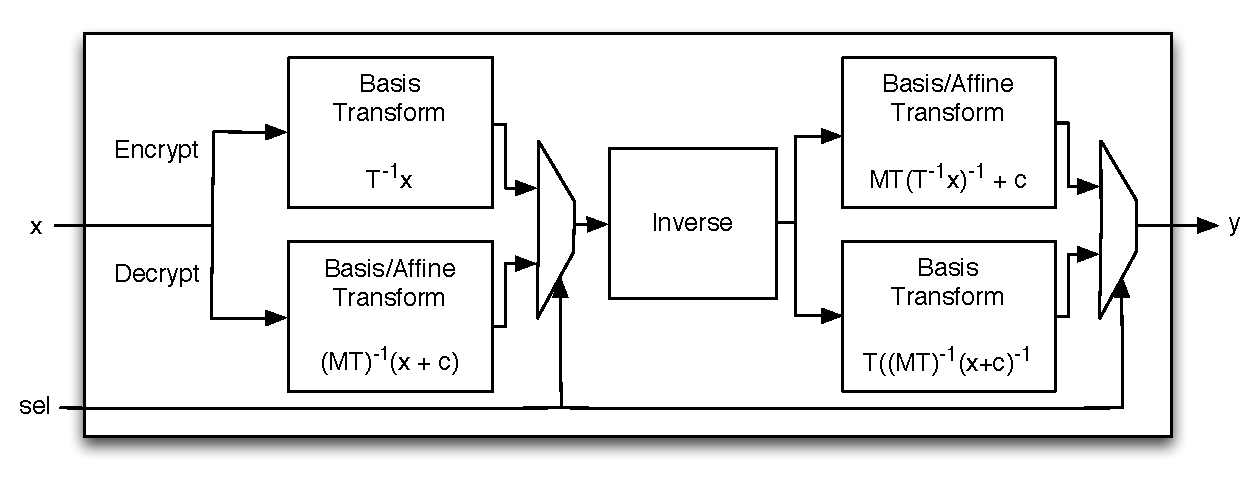
\includegraphics[scale=0.75]{./chapter_inverseImpl/merged_sboxes.pdf}
\caption{High-level diagram for a merged S-box circuit.}
\label{fig:merged}
\end{figure}

\section{Hardware Complexity}
Low-area hardware of these inversion circuits are most efficient when the basis change matrices have small weights (i.e. number of non-zero entries), as these correspond to a small number of logic gates required to perform the mappings. Since we are free to choose any basis for every subfield of $GF(2^{16})$, an exhaustive search for an optimal inversion circuit should generate all such bases and consider the complexity of the basis change transformation and the impact of the underlying arithmetic operations due to such selections. Algorithm \ref{alg:exhaustiveRootGeneration} presents the exhaustive search technique we used for finding all such mixed basis combinations. This could be greatly simplified by finding one root of each irreducible polynomial and then selecting its unique conjugate as the second root. However, we chose to be more thorough when finding all possible basis combinations. From these bases, we use the approach outlined in the previous sections to construct the basis change matrices and their respective inverses.

\begin{algorithm}[t] %[htb]
\caption{Exhaustive Basis Generation.} \label{alg:exhaustiveRootGeneration}
\begin{algorithmic}[1]
	\State $roots = []$
	\State $P(v) = v^2 + v + 1$
	\State Define $GF(2^2)$ with $P(v)$
	\State $pRoots = ZEROS(P)$
	\For{$\delta \in GF(2^2)$}
		\State $Q(w) = w^2 + w + \delta$
		\If{$Q(w)$ is irreducible}
			\State Define $GF((2^2)^2)$ with $Q(w)$
			\State $qRoots = ZEROS(Q)$
			\For{$\epsilon \in GF((2^2)^2)$}
				\State $R(x) = x^2 + x + \epsilon$
				\If{$R(x)$ is irreducible}
					\State Define $GF(((2^2)^2)^2)$ with $R(x)$
					\State $rRoots = ZEROS(R)$
					\For{$\zeta \in GF(((2^2)^2)^2)$}
						\State $S(y) = y^2 + y + \zeta$
						\If{$S(y)$ is irreducible}
							\State Define $GF((((2^2)^2)^2)^2)$ with $S(y)$
							\State $sRoots = ZEROS(S)$
							\For{each tuple $(p_r$, $q_r$, $r_r, s_r)$ for $P(v)$, $Q(w)$, $R(x)$, $S(y)$}
								\State $roots \gets Append(roots, (p_r,q_r,r_r,s_r))$
							\EndFor
						\EndIf
					\EndFor
				\EndIf
			\EndFor
		\EndIf
	\EndFor
	\State \Return $roots$
\end{algorithmic}
\end{algorithm}

Also, since we are programmatically generating these basis change matrices in Magma, we had to perform two basis changes to account for the fact that there is no support for normal basis arithmetic. More specifically, we first had to map elements in $GF(2^{16})$ represented in a polynomial basis to elements in $GF((((2^2)^2)^2)^2)$ represented in the tower of polynomial basesA $[1, V]$, $[1, W]$, $[1, X]$, and $[1, Y]$. Then, using the roots generated using Algorithm \ref{alg:exhaustiveRootGeneration}, we perform another mapping between the standard polynomial basis and the target mixed basis. However, rather than count the cost of both basis change matrices separately, we multiply them together to form a single matrix, which we effectively treat as $\mathbf{T}$ and $\mathbf{T}^{-1}$. 

% TODO: example with 2^8

For low-area combinational implementations of the S-box containing the inversion circuits, we measure the complexity, or cost, as the total number of gates required. To formulate this as an optimization problem, we first denote the set of all possible basis combinations as $\mathcal{B}$, where a particular element in this set is denoted as $\beta$. For example, a strictly polynomial basis element in this set can be $\beta = \{[1, V], [1, W], [1, X], [1, Y]\}$. We also define the set of all $2048$ degree-16 irreducible polynomials $T(z)$ over $GF(2)$ as $\mathcal{P}$. With these two sets, we let the function $Tr(\beta, T) : \mathcal{B} \times \mathcal{P} \to \{0,1\}^{256}$ be one that outputs the transformation (i.e. basis change matrix $\mathbf{T}$) given a particular set of basis elements and the polynomial $T(z)$ defining the field $GF(2^{16})$. The cost of each of these matrices is equal to the number of non-zero entries in each one. As such, we let $C_t(\mathbf{T}) : \{0,1\}^{256} \to \mathbb{N}$ be a function that returns the cost of a particular transformation matrix. With coefficients $\Sigma$, $\Pi$, and $\Lambda$ for $q(w)$, $r(x)$, and $s(y)$, respectively, we define the function $C_i(\beta, \Sigma, \Pi, \Lambda) : \mathcal{B} \to \mathbb{N}$ as one that returns the cost of the inverse calculation given a particular basis and set of coefficients. The cost of a particular S-box construction given a basis, coefficient set, affine transformation matrix $\mathbf{A}$, and constant $c$ that is not implemented as a merged design is then defined by the following cost function:
\begin{align*}
c(\beta, \Sigma, \Pi, \Lambda, T) = & C_t(Tr(\beta T)^{-1}) + C_t(\mathbf{A} \times Tr(\beta, T)) + C_t((\mathbf{A} \times Tr(\beta, T))^{-1}) + \\
& C_t(Tr(\beta, T)) + 2 \times (C_i(\beta, \Sigma, \Pi, \Lambda) + C(\mathbf{A}) + HW(c))
\end{align*}
If we follow the merged S-box design, then this cost function changes as shown below. We use $||$ to denote the concatenation of two $n \times n$ matrices together to form a single $2n \times n$ matrix.
\begin{align*}
c(\beta, \Sigma, \Pi, \Lambda, T) = & C_t(Tr(\beta, T)^{-1} || (\mathbf{A}\times Tr(\beta, T))^{-1}) + \\
& C_t(\mathbf{A\times Tr(\beta, T)} || Tr(\beta, T)) + C_i(\beta, \Sigma, \Pi, \Lambda) + 2 \times HW(c)
\end{align*}
Our goal of the \emph{exhaustive} search is to minimize these cost functions by considering all bases $\beta \in \mathcal{B}$, coefficients $\Sigma$, $\Pi$, and $\Lambda$, and the $GF(2^{16})$ field polynomial $T$. 

When considering all subfield polynomial and normal bases that have a trace of unity, there $128$ choices for $s(y)$, eight choices for $r(x)$, two choices for $q(w)$, and only one choice for $p(v)$ (see Appendix A for a list of all such polynomials). Since each of these polynomials has two distinct conjugate roots, where either one of the roots can be used to form a polynomial basis and both are required for a normal basis, there are three possible choices of a basis for elements in all subfields of $GF(2^{16})$ formed by degree $2$ extensions. Therefore, there is a total of $(128 \times 3) \times (8 \times 3) \times (2 \times 3) \times (1 \times 3) = 165888$ possible cases to consider for a single polynomial $T(v)$ that defines the field $GF(2^{16})$. Since the basis change matrices depend on the field representation of $GF(2^{16})$, and there are $4080$ degree $16$ irreducible polynomials, this means that we must consider $4080 \times 165888 = 676823040$ possible cases to find the minimal transformation. Unfortunately, this proved too much of a computational task to tackle for this work, so we selectively focused on the 21 smallest minimal polynomials $T(z)$ when searching for a $16$-bit S-box.


% Furthermore, since each basis change matrix is a linear map modulo $2$, we employ the logic optimization techniques discussed in Chapter \ref{chp:optimizeLinear}
% to minimize the number of XOR gates required for each implementation. Unlike Canright, our basis change matrices
% of $16 \times 16$ elements (and $32 \times 16$ for merged S-box designs) are too large 
% to perform an exhaustive factorization to find the minimal 
% cancellation-free linear circuit. Therefore, we take the best of Paar's greedy factorization technique and Boyar
% and Peralta's logic optimization method when tallying the final gate counts.

